\documentclass{article}

\usepackage{amsmath, amsthm, amssymb, amsfonts}
\usepackage{thmtools}
\usepackage{graphicx}
\usepackage{setspace}
\usepackage{geometry}
\usepackage{float}
\usepackage{hyperref}
\usepackage[utf8]{inputenc}
\usepackage[english]{babel}
\usepackage{framed}
\usepackage[dvipsnames]{xcolor}
\usepackage{tcolorbox}

%Define the listing package
\usepackage{listings} %code highlighter
\usepackage{color} %use color
\definecolor{mygreen}{rgb}{0,0.6,0}
\definecolor{mygray}{rgb}{0.5,0.5,0.5}
\definecolor{mymauve}{rgb}{0.58,0,0.82}
 
%Customize a bit the look
\lstset{ %
backgroundcolor=\color{white}, % choose the background color; you must add \usepackage{color} or \usepackage{xcolor}
basicstyle=\footnotesize, % the size of the fonts that are used for the code
breakatwhitespace=false, % sets if automatic breaks should only happen at whitespace
breaklines=true, % sets automatic line breaking
captionpos=b, % sets the caption-position to bottom
commentstyle=\color{mygreen}, % comment style
deletekeywords={...}, % if you want to delete keywords from the given language
escapeinside={\%*}{*)}, % if you want to add LaTeX within your code
extendedchars=true, % lets you use non-ASCII characters; for 8-bits encodings only, does not work with UTF-8
frame=single, % adds a frame around the code
keepspaces=true, % keeps spaces in text, useful for keeping indentation of code (possibly needs columns=flexible)
keywordstyle=\color{blue}, % keyword style
% language=Octave, % the language of the code
morekeywords={*,...}, % if you want to add more keywords to the set
numbers=left, % where to put the line-numbers; possible values are (none, left, right)
numbersep=5pt, % how far the line-numbers are from the code
numberstyle=\tiny\color{mygray}, % the style that is used for the line-numbers
rulecolor=\color{black}, % if not set, the frame-color may be changed on line-breaks within not-black text (e.g. comments (green here))
showspaces=false, % show spaces everywhere adding particular underscores; it overrides 'showstringspaces'
showstringspaces=false, % underline spaces within strings only
showtabs=false, % show tabs within strings adding particular underscores
stepnumber=1, % the step between two line-numbers. If it's 1, each line will be numbered
stringstyle=\color{mymauve}, % string literal style
tabsize=2, % sets default tabsize to 2 spaces
title=\lstname % show the filename of files included with \lstinputlisting; also try caption instead of title
}
%END of listing package%
 
\definecolor{darkgray}{rgb}{.4,.4,.4}
\definecolor{purple}{rgb}{0.65, 0.12, 0.82}
 
%define Javascript language
\lstdefinelanguage{JavaScript}{
keywords={typeof, new, true, false, catch, function, return, null, catch, switch, var, if, in, while, do, else, case, break},
keywordstyle=\color{blue}\bfseries,
ndkeywords={class, export, boolean, throw, implements, import, this},
ndkeywordstyle=\color{darkgray}\bfseries,
identifierstyle=\color{black},
sensitive=false,
comment=[l]{//},
morecomment=[s]{/*}{*/},
commentstyle=\color{purple}\ttfamily,
stringstyle=\color{red}\ttfamily,
morestring=[b]',
morestring=[b]"
}
 
\lstset{
language=JavaScript,
extendedchars=true,
basicstyle=\footnotesize\ttfamily,
showstringspaces=false,
showspaces=false,
numbers=left,
numberstyle=\footnotesize,
numbersep=9pt,
tabsize=2,
breaklines=true,
showtabs=false,
captionpos=b
}

\colorlet{LightGray}{White!90!Periwinkle}
\colorlet{LightOrange}{Orange!15}
\colorlet{LightGreen}{Green!15}

\newcommand{\HRule}[1]{\rule{\linewidth}{#1}}

\NewEnviron{NORMAL}{% 
    \scalebox{2}{$\BODY$} 
} 

\declaretheoremstyle[name=Theorem,]{thmsty}
\declaretheorem[style=thmsty,numberwithin=section]{theorem}
\tcolorboxenvironment{theorem}{colback=LightGray}

\declaretheoremstyle[name=Proposition,]{prosty}
\declaretheorem[style=prosty,numberlike=theorem]{proposition}
\tcolorboxenvironment{proposition}{colback=LightOrange}

\declaretheoremstyle[name=Principle,]{prcpsty}
\declaretheorem[style=prcpsty,numberlike=theorem]{principle}
\tcolorboxenvironment{principle}{colback=LightGreen}

\setstretch{1.2}
\geometry{
    textheight=9in,
    textwidth=5.5in,
    top=1in,
    headheight=12pt,
    headsep=25pt,
    footskip=30pt
}

% ------------------------------------------------------------------------------

\begin{document}

% ------------------------------------------------------------------------------
% Cover Page and ToC
% ------------------------------------------------------------------------------

\title{ \normalsize \textsc{}
		\\ [2.0cm]
		\HRule{1.5pt} \\
		\LARGE \textbf{\uppercase{Sistemi Operativi} \\
        Architetture e Sistemi Operativi - II Semestre
		\HRule{2.0pt} \\ [0.6cm] \LARGE{Corso A} \vspace*{10\baselineskip}}
		}
\date{\text{Ultima Compilazione - }\today}
\author{\textbf{Autore} \\ 
		Giuseppe Acocella \\
		2024/25\\
        \url{https://github.com/Peenguino}}
        

\maketitle
\newpage

\tableofcontents

%\begin{figure}[htbp]
    %\center
    %\includegraphics[scale=0.4]{img/classiComplessita2.png}
%\end{figure}


\newpage

\section{Caching}

Il Caching ha come obiettivo quello di astrarre sulle gerarchie di memoria e creare l'\textbf{illusione} di avere la stessa quantità di memoria "lenta" ma alla velocità della memoria "veloce". Questo è solo un esempio che cerca di illustrare l'obiettivo del caching.
Si vuole creare una gerarchia di memorie, classificate per velocità e "vicinanza" alla CPU, permettendo l'accesso a dati ricorrenti in tempo breve.

\subsection{Gerarchia di Memorie}

Classifichiamo le memorie secondo la loro velocità. Più veloci saranno e più saranno costose e piccole in termini di spazio in $byte$.
Oltre a questo dobbiamo tenere in considerazione 
il modo in cui si stanno evolvendo le CPU e le memorie:

\begin{figure}[htbp]
    \center
    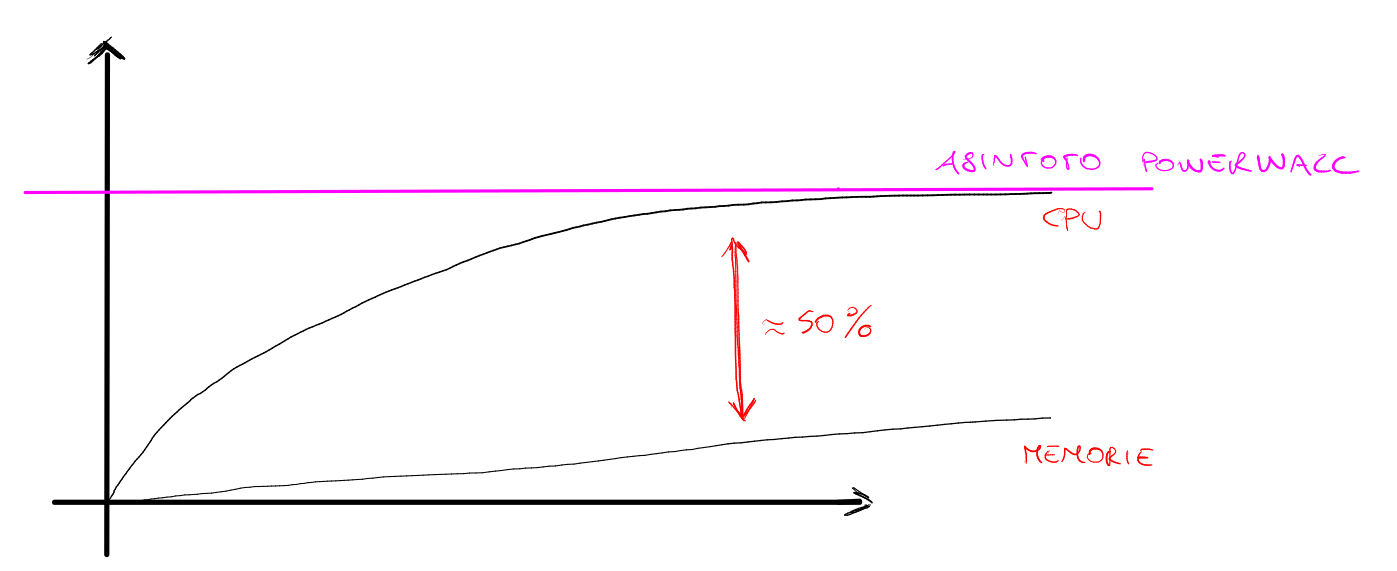
\includegraphics[scale=0.25]{img/rapporto_CPU_mem.png}
\end{figure}

Questo è un altro motivo per cui si vuole gestire in maniera più intelligente la comunicazione tra processore e memoria.

\paragraph{Istanza di Caching} Assumiamo di avere quattro memorie:
\[ A1,\:\:A2,\:\:A3,\:\:A4 \]
Ed ognuna di queste memorie sarà caratterizzata da un tempo, ordinate in tempo crescente:
\[ T_{A1},\:\:T_{A2},\:\:T_{A3},\:\:T_{A4} \]
E' necessario tenere in considerazione come modello di riferimento quello di \textit{Von Neumann}, di conseguenza abbiamo una \textbf{CPU} che interagisce con una \textbf{memoria} grazie ad un canale di comunicazione. Spesso l'utilizzo di questo canale causa un effetto di \textbf{bottleneck}. Si vuole quindi trovare un compromesso che possa velocizzare la comunicazione tra \textbf{CPU} e \textbf{memoria}. Le prestazioni di una memoria dipendono fortemente dalla tecnologia del supporto\footnote{La classificazione di tecnologia delle memorie è presente nel primo modulo di appunti: Architetture degli Elaboratori.}.
\newpage

Illustriamo la gerarchia delle memorie e la loro "distanza" dalla CPU.

\begin{figure}[htbp]
    \center
    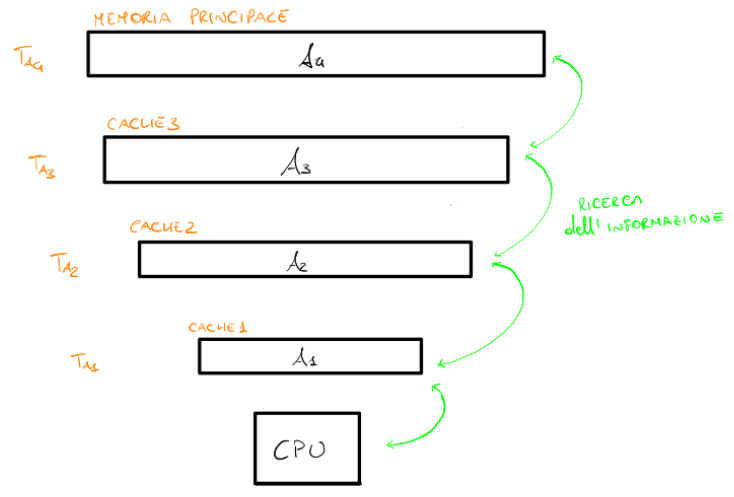
\includegraphics[scale=0.42]{img/gerarchiaMemorie.png}
\end{figure}

Possiamo assumere queste tempistiche delle memorie:
    \[ T_{A_{1}} = 4 \tau \: \: \: \: T_{A_{2}} = 10 \tau\]
    %\vspace{-px}
    \[ T_{A_{3}} = 20 \tau \: \: \: \: T_{A_{4}} = 60/80\:nsec \]

\subsection{Hit/Miss Rate, Miss Penalty, AMAT}

Una volta impostata la gerarchia rappresentata sopra, è necessario capire se un \textbf{indirizzo} dato sia o meno presente ad uno specifico \textbf{livello} tra quelli illustrati. 

\begin{enumerate}
    \item \textbf{Hit Rate}: Percentuale di "Hit", ossia dati \textbf{trovati}.
    \item \textbf{Miss Rate}: Percentuale di "Miss", complementare a quella di "Hit", ossia dati \textbf{non trovati}.
    \item \textbf{Miss Time}: Tempo impiegato per effettuare la fetch con esito di "Miss".
    \item \textbf{Miss Penalty}: Tempo impiegato per risalire la gerarchia delle cache fino al ritrovamento del dato cercato.
    \item \textbf{AMAT}: Average Memory Access Time: 
    \[ AMAT\: = \: HIT\_TIME \: + \:( MISS\_RATE \: * \: MISS\_PENALTY) \]
\end{enumerate}

La differenza tra \textbf{Miss Time} e \textbf{Miss Penalty} può variare anche di ordini di grandezza. L'\textbf{Hit Rate} deve essere superiore al $90\%$ per rendere efficiente lo schema delle cache così impostate.

\newpage

\subsection{Principio di Località}

Risulta necessario stabilire il criterio con il quale vengono caricati questi blocchi di memoria più performanti e vicini alla CPU. Le informazioni caricate sulla cache seguono il cosiddetto \textbf{principio di località}:

\begin{enumerate}
    \item \textbf{Località Spaziale}: Solitamente per un certo periodo di tempo, molti dati potrebbero risultare vicini tra di loro. In questo caso si stabilisce quindi la grandezza di un blocco e questo verrà caricato tutto sulla cache. Questo permetterà probabili accessi successivi in tempi ridotti, anche di svariati ordini di grandezza.
    Secondo questo principio, accedendo a $M[PC]$, molto probabilmente accederò a $M[PC+4]$, $M[PC+8]$ ... 
    \item \textbf{Località Temporale}: Spesso un dato corrente potrebbe essere riutilizzato in breve tempo. Di conseguenza si preferisce mantenere il dato in cache. Secondo questo principio, accedendo a $M[PC]$, probabilmente in breve tempo potrei riaccedere a $M[PC]$.
\end{enumerate}

Grazie a questo principio si stabilisce il criterio con cui vengono caricati i blocchi in cache. Questo procedimento permette in $1\tau$\footnote{Tempo breve generico, abbiamo assunto un ciclo di clock, per rendere l'idea che un blocco viene caricato tutto sulla cache in un singolo tempo, essendo appunto in "blocco".} di caricare in cache un blocco di grandezza arbitraria. E' necessario ricordare che questi principi possono essere applicati a tutti i tipi di dato (codice oppure effettivo dato in memoria).

\subsection{Tempi CPU (CPI e Miss Penalties)}

Elenchiamo diverse formule di calcolo dei tempi CPI (clock per instructions), illustrando anche l'influenza su questi tempi delle penalties causate dalle informazioni non trovate nella cache.

\[ CPU_{TIME} \: = \: (CPI_{PERFECT} \: + CPI_{MISS\_PENALTY}) \: * \: LEN\_CICLO\_CLOCK  \]
\vspace*{-10px}
\[ CPI_{PERFECT} \: = \: \frac{IC_{CPU}}{IC}CPI_{CPU} \: + \: \frac{IC_{MEM}}{IC}CPI_{MEM}\]
\vspace*{-10px}
\[ CPI_{MISS\_PENALTY} \: = \: \frac{IC_{MEM}}{IC} \: * \: MISS\_RATE \: * \: MISS\_PENALTY  \]
\vspace*{-10px}
\[ CPI_{STALL} = CPI_{STALL\_IST} \: + \: CPI_{STALL\_DATA} \]
\vspace*{-10px}
\[ CPI \: = \: CPI_{PERFECT} \: + \: CPI_{STALL} \]
\vspace*{-10px}
\[ CPI_{STALL} = MISS\_RATE_{IST} \: \:*  \: \: MISS\_PENALTY\]
\vspace{5px}

L'identificatore $IC$ corrisponde al contatore di istruzioni. Un caching efficiente tende a minimizzare la percentuale di miss rate. Questa minimizzazione spesso è forzata da tecniche di \textbf{prefetching}, ossia si manda in background il caricamento della cache cercando di "prevedere" i dati che verranno utilizzati in caso siano validi i principi di località.

\newpage

\subsection{Tipi di Indirizzamento}

Abbiamo definito i criteri e l'organizzazione fisica del caching. Ma non abbiamo ancora definito come possiamo effettivamente trovare/non trovare un determinato indirizzo dato in cache. Se assumiamo che la cache sia un sottoinsieme della memoria principale, allora abbiamo la certezza (conoscendo le dimensioni di entrambe le memorie citate) che degli indirizzi possono collidere. Sicuramente almeno due indirizzi della memoria principare avranno la stessa locazione in cache. Di conseguenza elenchiamo tre tipi di indirizzamento caratterizzati da proprietà diverse.

\vspace*{15px}

\paragraph{Working Set} Insieme di istruzioni/dati consecutivi in un certo intervallo di tempo. \newline L'analisi della località di questi set permette la gestione logica delle cache.

\begin{figure}[htbp]
    \center
    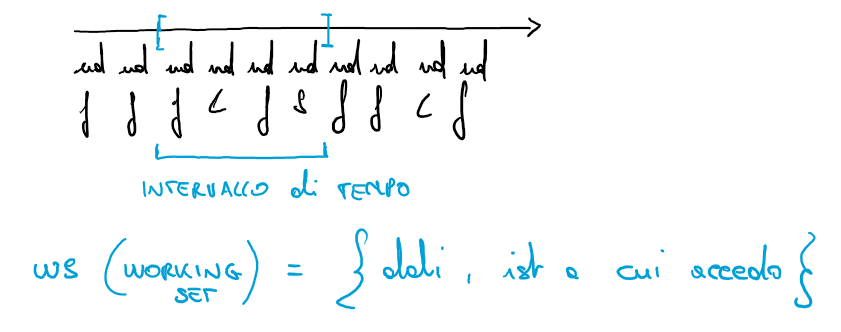
\includegraphics[scale=0.50]{img/workingSet.png}
\end{figure}

\subsubsection{Indirizzamento Diretto}

Immaginiamo di avere una memoria principale di dimensioni $N$, la cache a disposizione della CPU sarà invece di dimensioni $N^{I}$ con $N >> N^{I}$. Alla base dell'indirizzamento diretto c'è l'interpretazione di parte dell'indirizzo cercato come \textbf{tag} da cercare nelle linee della cache. 

\begin{figure}[htbp]
    \center
    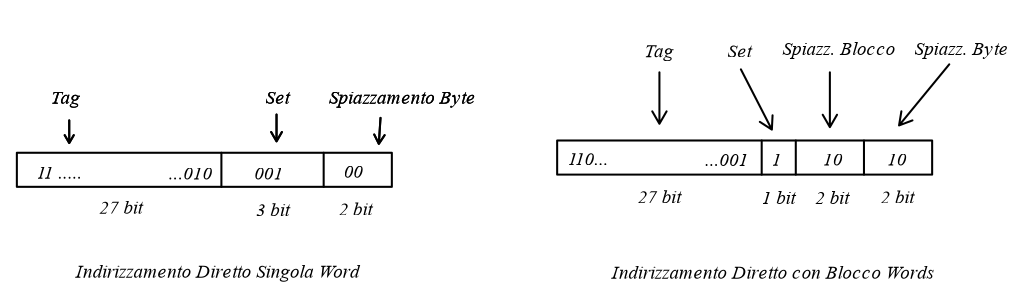
\includegraphics[scale=0.425]{img/indirizzamento_diretto_indirizzi.png}
\end{figure}

\paragraph{Trashing} A causa delle differenze di dimensioni tra memoria e cache, sicuramente più indirizzi avranno la stessa chiave, di conseguenza se dovesse capitare di dover caricare in cache più indirizzi con la stessa chiave si andrebbe in contro ad un continuo \textbf{caricamento} e \textbf{scaricamento} di dati tra la cache e la memoria. Questo fenomeno è detto \textbf{trashing} ed è un punto di debolezza delle cache ad indirizzamento diretto. Effettuare questi spostamenti continui di dati invaliderebbe infatti tutti i vantaggi ottenuti dall'utilizzo delle cache.

\vspace*{5px}

Mostriamo a pagina successiva la logica di questo tipo di indirizzamento e la sua implementazione fisica su rete combinatoria.

\newpage

\begin{enumerate}
    \item \textbf{Implementazione Logica}: Mostriamo uno schema della logica dietro \newline l'indirizzamento diretto ed analizziamolo a step.
    \begin{figure}[htbp]
        \center
        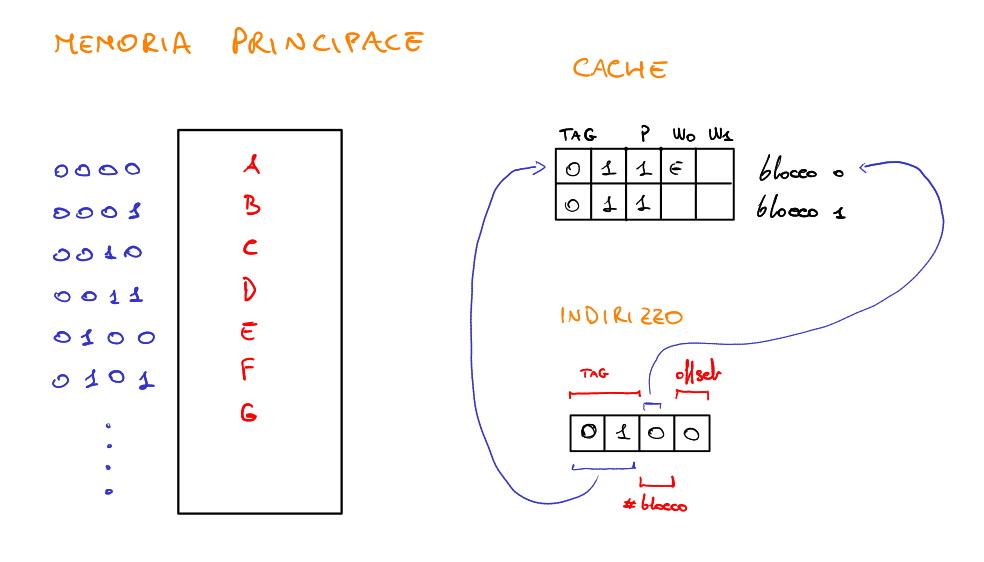
\includegraphics[scale=0.375]{img/ind_diretto_logico.png}
    \end{figure}
    \begin{enumerate}
        \item Ogni dato in memoria avrà un \textbf{indirizzo}. Assumiamo un indirizzo composto da $4$ bit e diamo un interpretazione alle cifre.
        \item Ogni indirizzo sarà dunque composto da un \textbf{tag} (bit 0-1), un \textbf{blocco} (bit 2) e da un \textbf{offset} (bit 3).
        \item Nella cache saranno presenti vari blocchi (linee) e ciascuna di queste avrà un \textbf{tag}, un \textbf{bit di presenza} (p) e varie \textbf{word}, se saranno selezionabili grazie all'\textbf{offset} determinato dall'indirizzo cercato. 
    \end{enumerate}
    \item \textbf{Implementazione Fisica}: Mostriamo la rete combinatoria dietro l'indirizzamento diretto ed analizziamola a step.
    \begin{figure}[htbp]
        \center
        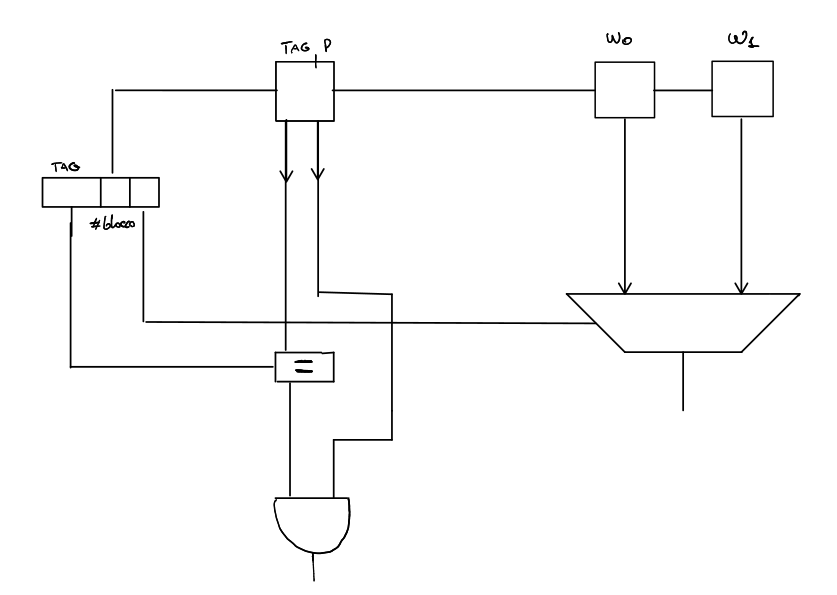
\includegraphics[scale=0.325]{img/ind_diretto_fisico.png}
    \end{figure}
    \begin{enumerate}
        \item Tre moduli rappresentanti la cache, il primo mantiene le informazioni riguardanti il \textbf{tag} ed il \textbf{bit di presenza}.
        \item L'indirizzo in input è interpretato come nell'implementazione logica.
        \item Il confrontatore prende in input il tag dell'indirizzo in ingresso ed il tag della cache.
        \item La porta \textbf{AND} produce in output l'esito di \textbf{hit/miss}, mentre il multiplexer permette di selezionare la word cercata, se presente.
    \end{enumerate}
\end{enumerate}

\newpage

\subsubsection{Indirizzamento Associativo}

Questo tipo di indirizzamento interpreta parte dell'indirizzo in ingresso come chiave e dedica, ad ogni possibile chiave, una linea di cache. Questo permette di avere una cache molto flessibile e non presenterà problemi causati dalle collisioni. Questa gestione della cache però è davvero costosa, dato che saranno presenti un numero molto alto di confrontatori. Mostriamo le implementazioni di questo schema di cache:

\vspace*{15px}

\begin{enumerate}
    \item \textbf{Implementazione Logica}: Illustriamo la gestione delle linee di cache e dell'indirizzo in ingresso.
    \begin{figure}[htbp]
        \center
        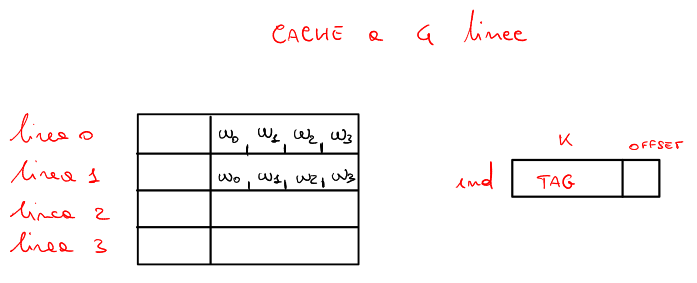
\includegraphics[scale=0.5]{img/ind_associativo_logico.png}
    \end{figure}
    \begin{enumerate}
        \item Ogni cache avrà due colonne, la prima rappresenterà i \textbf{tag} mentre la seconda le $kword$ per ogni linea.
        \item Ogni indirizzo avrà quindi una corrispondente linea in cache, e la word singola in output sarà determinata dalla parte di \textbf{offset}.
    \end{enumerate}

    \vspace*{15px}
    
    \item \textbf{Implementazione Fisica}: Illustriamo l'implementazione fisica di una \textbf{singola} linea di cache.
    \begin{figure}[htbp]
        \center
        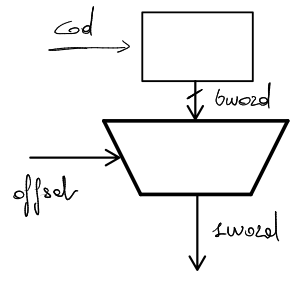
\includegraphics[scale=0.5]{img/ind_associativo_fisico.png}
    \end{figure}
    \vspace*{15px}
    \newline
    Questa illustrazione permette di capire il costo di questa gestione della cache. Ogni \textbf{singola linea} di cache richiederà un \textbf{confrontatore} ed un multiplexer. Solitamente una cache contiene una quantità di linee che si aggira sull'\textbf{ordine delle migliaia}.
\end{enumerate}

\newpage

\subsubsection{Indirizzamento Set Associativo}

Le due precedenti gestioni di cache offrivano pro e contro. Di conseguenza si preferisce un ibrido tra indirizzamento diretto ed associativo, in modo tale da poter bilanciare rispettivamente sia i problemi causati dalle collisioni sia i costi eccessivi. Illustriamo la gestione di questo tipo di indirizzamento:

\begin{enumerate}
    \item \textbf{Implementazione Logica}: Descriviamo per step il funzionamento di questo schema:

    %\begin{figure}[htbp]
    %    \center
    %    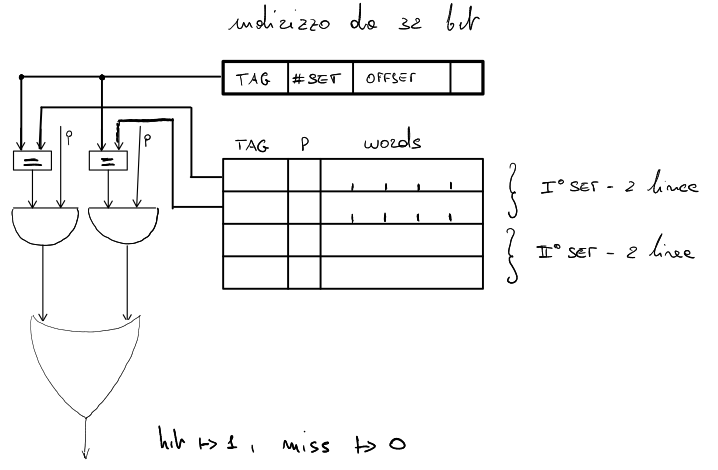
\includegraphics[scale=0.5]{img/ind_set_associativo_logico.png}
    %    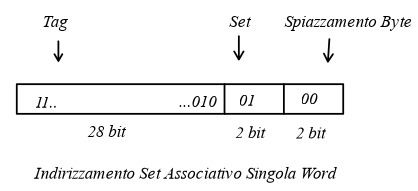
\includegraphics[scale=0.5]{img/indirizzamento_diretto_indirizzi2.png}
    %\end{figure}
    
\begin{figure}[H]
  \centering
  \begin{minipage}[b]{0.4\textwidth}
    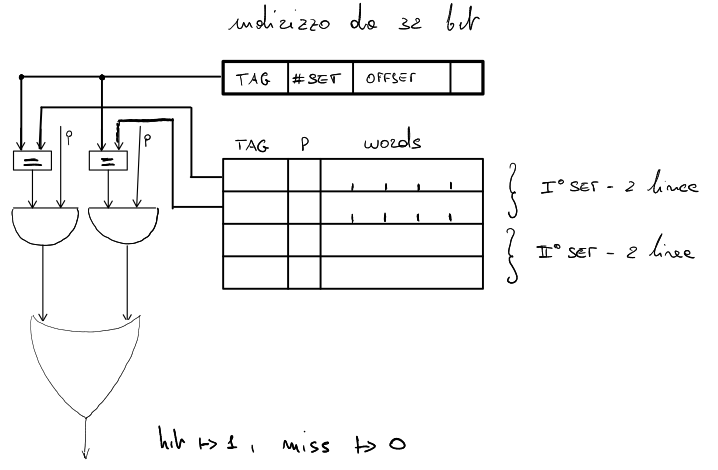
\includegraphics[width=\textwidth]{img/ind_set_associativo_logico.png}
  \end{minipage}
  \hspace{10px}
  \begin{minipage}[b]{0.4\textwidth}
    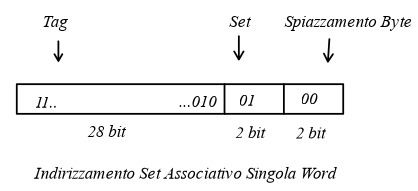
\includegraphics[width=\textwidth]{img/indirizzamento_diretto_indirizzi2.png}
  \end{minipage}
\end{figure}

    \begin{enumerate}
        \item Ogni \textbf{indirizzo} in \textbf{ingresso} sarà interpretato con \textbf{tag}, \textbf{numero set} ed \textbf{offset}.
        \item Le \textbf{linee} di cache vengono raggruppati in \textbf{set}. Di conseguenza si effettua un indirizzamento \textbf{associativo} sul \textbf{set} di appartenenza.
        \item Una volta selezionato il \textbf{set} si effettua un indirizzamento \textbf{diretto} utilizzando il \textbf{tag} tra le varie linee del \textbf{set} corrente.
        \item Infine, se si ha un segnale di \textbf{hit}, allora si utilizza l' \textbf{offset} per ricavare la \textbf{singola word} tra le \textbf{kword}.
    \end{enumerate}

    \item \textbf{Implementazione Fisica}: Descriviamo la composizione di questa rete di una cache a $2$ vie.

    \begin{figure}[htbp]
        \center
        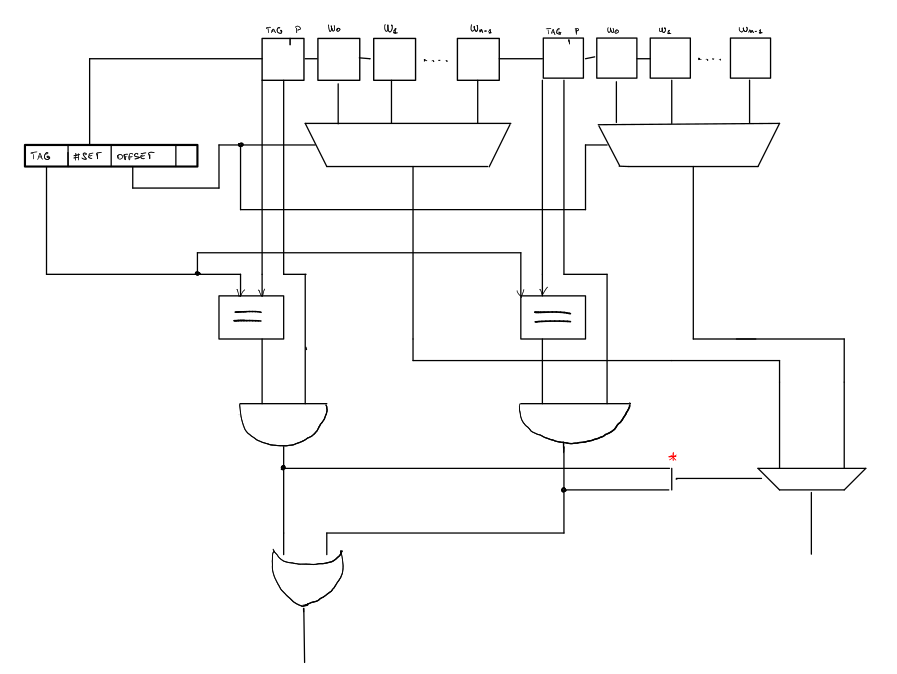
\includegraphics[scale=0.3]{img/ind_set_associativo_fisico.png}
    \end{figure}

    \begin{enumerate}
        \item Ogni via è caratterizzata da un modulo contenente \textbf{tag} e \textbf{bit} di \textbf{presenza} ed i restanti le \textbf{word} di quella linea.

        \newpage
        
        \item L'\textbf{indirizzo} in ingresso è caratterizzato da \textbf{tag}, \textbf{numero} di \textbf{set} ed \textbf{offset}.
        \item Tutti i moduli contenenti \textbf{word} danno in input ad un \textbf{multiplexer} il loro contenuto, il cui segnale di controllo è rappresentato dall'\textbf{offset} dell'\textbf{indirizzo} in ingresso.
        \item Viene utilizzato un numero di comparatori pari al numero di \textbf{set}, questi avranno in input il \textbf{tag} del primo modulo del corrente \textbf{set} ed il \textbf{tag} dell'\textbf{indirizzo} in \textbf{ingresso}.
        \item Delle porte \textbf{AND} prendono in ingresso il \textbf{bit} di \textbf{presenza} e l'output dei \textbf{comparatori} per ogni \textbf{set} e producono un segnale di \textbf{hit/miss} entrando in una porta \textbf{OR}.
        \item Infine, l'output delle porte \textbf{AND} viene portato ad un multiplexer come segnale di controllo, permettendo la scelta tra le uscite dei \textbf{multiplexer} di \textbf{ciascun set}. In questo particolare caso non è necessario utilizzare un codificatore prima dell'ingresso di controllo sull'ultimo multiplexer in basso, essendo il caso di soli due set, altrimenti sarebbe stato necessario anche quel componente.
    \end{enumerate}
    
\end{enumerate}

\vspace*{15px}

\paragraph{Confronto Caratteristiche Indirizzamenti} Riassumiamo le caratteristiche di ciascun tipo di indirizzamento sopra illustrato:

\vspace*{20px}

\begin{center}
\begin{tabular}{ |c|c c| } %|c|c|c|%
 \hline
  & \#vie & \#insiemi \\ 
 \hline
 diretto & 1 & \#linee cache \\ 
 associativo & \#linee cache & $1$ \\
 set associativo & \#vie & $\frac{\#linee}{\#vie}$ \\
 \hline
\end{tabular}
\end{center}

\vspace*{15px}

\subsection{Accenni di Gestione Stalli Miss Penalties}

Nel momento in cui accade una \textbf{miss penalty} il processore entra in \textbf{stallo} per un periodo di tempo abbastanza ampio. Per questo motivo si preferisce attuare delle politiche grazie alle quali si "nasconde" il tempo di stallo in questione:

\begin{enumerate}
    \item \textbf{Out of Order Execution}: Si eseguono operazioni future non in ordine e che permettano di non invalidare le Condizioni di Bernstein.
    \item \textbf{Esecuzione Speculativa Salti}: Si prevede un salto, assumendo che porti a qualcosa di già fatto.
    \item \textbf{Prefetching}: Si cerca di prevedere cosa verrà caricato in cache, avviando veri e propri caricamenti in cache in \textbf{background}. Questo non sempre può essere realizzato, ma quando possibile permette un efficace minimizzazione degli stalli causati dalle miss penalty.
\end{enumerate}

\newpage

\subsection{Tipologie di Miss}

I \textbf{miss} si dividono in \textbf{specifiche categorie} rispetto alla "causa" che li genera:

\begin{enumerate}
    \item \textbf{Fisiologici}: Cronologicamente il primo miss necessario al caricamento della cache.
    \item \textbf{Capacità}: La grandezza del \textbf{Workspace} supera quella della \textbf{cache}.
    \item \textbf{Conflitto}: Causato dal tipo di indirizzamento. Questa tipologia può essere risolta a tempo di compilazione.
\end{enumerate}

\subsection{Scrittura in Cache}

Elenchiamo tutte le caratteristiche e le problematiche della scrittura in cache e della sua consistenza in relazione ai dati presenti in memoria principale.

\subsubsection{Problemi in Scrittura}

Elenchiamo le possibili problematiche causate dalla scrittura in cache:

\begin{enumerate}
    \item \textbf{Scrittura 1 word/b word}: Assumiamo di avere un indirizzo su cui vogliamo effettuare una $STR$ in una cache set associativa a $2$ vie. Non posso semplicemente scrivere il \textbf{dato (singola word)} e segnare a quella linea il bit di presenza ad $1$ perché starei sprecando tutte le $b-1$ word presenti in quella linea su cui potrei ancora scrivere. Dunque si effettua lo stesso procedimento delle $LDR$, favorendo il caricamento di tutti i dati adiacenti a quello corrente nella linea di cache.
    
    \begin{enumerate}
        \item \textbf{Eccezione}: Questo comportamento può causare problematiche nel caso in cui si voglia inizializzare un array con elementi arbitrari (da modificare successivamente) al suo interno. In quel caso non avrebbe senso caricare in cache tutti i dati, dato che verrebbero riscritti poco dopo. Questi tipi di ottimizzazioni vengono controllate dal compilatore, se è in grado di accorgersi di queste problematiche.
    \end{enumerate}
\end{enumerate}

\subsubsection{Inconsistenza Cache/Memoria - Write Back/Write Through}

La scrittura in cache causa un altro tipo di problematica, ossia la \textbf{consistenza} dei dati in \textbf{cache} ed in \textbf{memoria principale}. Tutte le locazioni paralleli dovrebbero essere "informate" di una potenziale modifica. Esistono $2$ approcci diversi che risolvono questa problematica:

\begin{enumerate}
    \item \textbf{Strategia Write Back}: Si aggiunge un nuovo \textbf{bit flag} alle linee di cache, ossia $M \in \{ 0,1 \}$, se il contenuto della linea è stato modificato allora la flag va ad $1$, altrimenti resta a $0$. Sarà dunque necessario ad un certo punto un "refresh" della memoria, trasportando tutti i dati modificati ai livelli superiori.
    \item \textbf{Strategia Write Through}: Non utilizzo un bit flag, ma ogni modifica effettuata in cache viene messa in coda ad un \textbf{buffer} e l'aggiornamento dei livelli superiori avverrà in maniera \textbf{asincrona}. Questo approccio dipende fortemente dalla dimensione del buffer, questo dovrà essere abbastanza grande da contenere tutte le modifiche in coda fino all'effettivo refresh.
    \newpage
    \item \textbf{Strategia Write Back Bufferizzata}: Versione asincrona del write back, si compone di queste fasi:
    \begin{enumerate}
        \item Si copia la modifica nel buffer di scrittura.
        \item Senza attendere la fase precedente, carico le $b$ parole nuove in cache.
        \item Finisce l'accesso in cache.
    \end{enumerate}
\end{enumerate}

\subsection{Politiche di Rimpiazzamento - Sequenziale/LRU}

Che criterio segue ogni tipologia di indirizzamento di cache nel caso in cui bisogna aggiungere un nuovo dato in una cache già piena?

\begin{enumerate}
    \item \textbf{Indirizzamento Diretto}: Viene sostituita in maniera secca la linea di cache a cui sta facendo riferimento il nuovo indirizzo.
    \item \textbf{Indirizzamento Associativo}: Dato che questo tipo di indirizzamento non provocava collisioni, siamo costretti a scegliere una "vittima" in cache da sostituire con l'indirizzo corrente, essendo certi di aver finito lo spazio.
    \item \textbf{Indirizzamento Set Associativo}: Viene scelta una "vittima" da sostituire come nel caso precedente ma in uno specifico set.
\end{enumerate}

Il focus diventa quindi la gestione del \textbf{working set}, in modo tale da ottimizzare il caricamento/scaricamento delle cache in relazione al corrente working set.

\begin{enumerate}
    \item \textbf{Politica Sequenziale - Indirizzamento Diretto}: Questo approccio è quello più semplice possibile, infatti dopo il primo miss in cache si carica in cache un blocco di $b$ words. Appena sarà richiesta una word fuori da quel blocco viene effettuato un nuovo caricamento di blocco di words in cache.
    \item \textbf{Politica LRU\footnote{LRU sta per Least Recent Used, dunque utilizzato meno recentemente.} Puro - Indirizzamento Set Associativo}: L'idea è quella di mantenere un tempo di accesso $t_{a}$ per sostituire quello che servirà tra più tempo. Questo porta però ad un costo molto alto, dato che per ogni linea andrebbe controllato il tempo "mancante" al prossimo accesso. Si preferisce quindi un compromesso, ossia l'LRU Approssimato.
    \item \textbf{Politica LRU Approssimato - Indirizzamento Set Associativo}: Ogni linea di cache si porta dietro una flag d'accesso $A \in \{ 0,1 \}$ che viene alzata ad ogni accesso a quella linea. Ogni $k$ cicli di clock viene effettuata un operazione di \textbf{azzeramento}, dove tutte le $A$ vengono portate a $0$. Questa logica non è molto costosa dal punto di vista implementativo, ma è fortemente influenzata dall'ampiezza del periodo di refresh, dato che un periodo troppo lungo porterebbe a troppi bit $A=1$, mentre troppo breve porterebbe alla scelta random di locazioni.
\end{enumerate}

\newpage

\subsection{Cache Coherence}

Assumiamo di essere in un contesto multicore, dove ciascun core dispone di almeno un livello di cache completamente dipendente dal core stesso. La gestione concorrente dell'esecuzione complessiva dei programmi va attentamente gestita, dato che facilmente può crearsi inconsistenza tra copie dello stesso dato in cache di core diversi.

\paragraph{Mantenimento Coerenza} Abbiamo bisogno di due meccanismi per mantenere la coerenza delle cache:

\begin{enumerate}
    \item Meccanismo di \textbf{tracciamento} copie di un determinato dato $x$ in tutte le cache.
    \item Meccanismo di \textbf{informazione} a tutte le copie di un dato $x$ sulla \textbf{modifica} apportata. Potenzialmente esistono due approcci:
    \begin{enumerate}
        \item Propagazione del nuovo valore di $x$ a tutte le copie in tutte le cache.
        \item Invalidazione di tutte le altre copie di $x$.
    \end{enumerate}
\end{enumerate}

\subsubsection{Cache Coherence Protocols}

Esistono due protocolli che permettono la sincronizzazione dei dati tra tutte le cache di primo livello dei vari core. Elenchiamoli:

\begin{enumerate}
    \item \textbf{Snoopy Based}: Tutti i core sono in ascolto su un \textbf{bus}, quando un \textbf{core} effettua una \textbf{write} in una sua \textbf{cache} manda un segnale sul \textbf{bus} che permette una sincronizzazione tra tutti i core.
    \item \textbf{Directory Based}: Si mantiene una \textbf{tabella} nel primo livello di \textbf{cache comune} tra tutti i core che contiene tutte le informazioni sui dati e sulle locazioni di tutte le sue copie. In questo modo, utilizzando questa \textbf{mappa} è possibile \textbf{sincronizzare} tutte le copie nelle varie \textbf{cache.}
\end{enumerate}

Ogni tipo di protocollo scelto influisce sull'\textbf{AMAT} complessivo.

\subsubsection{False Sharing}

In specifici contesti, questi protocolli di sincronizzazione causano una quantità molto grande di operazioni "inutili" derivate dalla logica alla base della coerenza implementata in questo modo. Mostriamo un esempio:

\vspace*{12px}

\begin{enumerate}
    \item Assumiamo di avere un array molto grande, sull'ordine dei $k$ in grandezza.
    \vspace*{12px}
    \item Assumiamo di avere una macchina con $4$ core, suddividiamo l'array in quattro parti e ciascun core calcolerà la somma di ogni quarto di array, depositando il risultato in una specifica posizione di un array risultato di $4$ posizioni.
    \newpage
    \item Ogni core caricherà in cache una copia dell'array risultato e cercheranno di sincronizzare tutti i valori di quest'ultimo ad ogni operazione effettuata. Ma impostato in questo modo, l'array risultato è "impropriamente condiviso", infatti ogni core si occupa di \textbf{una sola} cella. Questo fenomeno è detto \textbf{false sharing} ed è un effetto collaterale della \textbf{cache coherence} che causa inutile traffico di sincronizzazione non desiderato. Una soluzione è quella di posizionare, grazie al \textbf{padding}, i risultati di ciascun core in memoria che \textbf{non risulti} condivisa.
\end{enumerate}

\section{Gestione I/O e Periferiche}

Per rendere un calcolatore in grado di acquisire dati dall'interno/esterno è necessario gestire l'\textbf{I/O}. Assumiamo che un programma impiega un tempo $t$ per terminare. Considerando quest'ultimo, si aggiunge circa un $\frac{1}{10}t$ al tempo complessivo.
Un concetto fondamentale è anche quello della differenza tra la velocità delle operazioni di I/O e la velocità di esecuzione delle istruzioni della CPU. E' fondamentale che non si crei un collo di bottiglia al processore alla velocità delle operazioni di I/O, la CPU deve essere in grado di eseguire altre istruzioni mentre lavorano le periferiche esterne.

\subsection{Legge di Amdahl}

Questa legge stabilisce il rapporto "all'infinito" del tempo parallelizzabile e non parallelizzabile, in questo caso rispettivamente tempo generico di esecuzione della \textbf{CPU} e tempo dedicato all'\textbf{I/O}.

\[ T_{seq} = fT_{seq} + (1-f)T_{seq} =\]

\[ \lim_{x\xrightarrow{}\infty} \frac{T_{seq}}{fT_{seq} + \frac{(1-f)T_{seq}}{n}} = \]

\vspace*{5px}

\[ = \frac{T_{seq}}{fT_{seq}} = \frac{1}{f} \]

\vspace*{5px}

\subsection{Prima Descrizione Gestione I/O}

Ogni genere di dispositivo di I/O ha la necessità di gestire:

\begin{enumerate}
    \item \textbf{Controllo}: Gestione degli ordini e dei segnali per gli esiti.
    \item \textbf{Dati}: Dati di input/output.
\end{enumerate}

Descriviamo sommariamente i passi necessari alla comunicazione tra \textbf{CPU} e device \textbf{I/O}:

\begin{enumerate}
    \item CPU controlla stato periferica, l'I/O risponde al controllo.
    \item CPU se e solo se il dispositivo è libero manda il comando alla periferica.
    \item Periferica esegue l'istruzione.
    \newpage
    \begin{enumerate}
        \item Se c'è necessità di trasferimento dati alla CPU viene eseguito in questo momento.
    \end{enumerate}
    \item I/O "fa rapporto" sull'esito dell'operazione appena eseguita.
\end{enumerate}

\vspace*{10px}

\paragraph{Device I/O} La comunicazione del device in maniera approssimativa si mostra in questo modo:

\begin{figure}[htbp]
    \center
    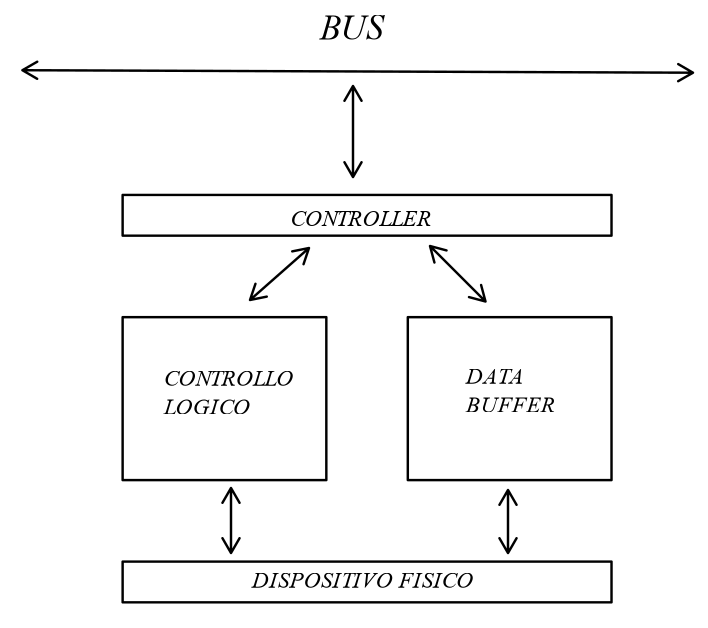
\includegraphics[scale=0.4]{img/device_io1.png}
\end{figure}

La rappresentazione del buffer è \textbf{approssimativa}, infatti non dobbiamo pensare che sia un semplice cavo da $1$ bit, ma un vero e proprio \textbf{insieme di cavi} che permettono il trasporto d'informazioni riguardo \textbf{indirizzo}, \textbf{controllo}, \textbf{dati} ed \textbf{arbitraggio}.

Due \textbf{tipologie} comuni di \textbf{bus} sono ad esempio \textbf{USB} o \textbf{PCIe}.

\vspace*{15px}

\paragraph{Comunicazioni sul Bus} Il bus è condiviso, le informazioni vengono dunque inviate in broadcast a tutti i device, ogni dispositivo però potrebbe avere clock diversi:

\begin{enumerate}
    \item \textbf{Gestione Sincrona}: Il clock è uno solo ed ogni device si adatta a quest'ultimo.
    \item \textbf{Gestione Asincrona}: Ogni device ha un proprio clock, generando un effetto \textbf{skewed}. Questo fenomeno va "ammortizzato" cercando di generare sincronizzazione solo ad uno specifico momento di comunicazione tra dispositivi e CPU.
\end{enumerate}

\newpage

\subsection{Protocolli di Arbitraggio del Bus}

Dopo aver definito il \textbf{bus} come mezzo di \textbf{comunicazione condiviso} tra tutti i dispositivi, è necessario stabilire come questi ultimi vengano arbitrati in modo tale da \textbf{non operare} in \textbf{conflitto} tra loro.

\vspace*{12px}

\begin{enumerate}
    \item \textbf{Daisy Chaining}: Sul bus è settata una priorità per device:
    \begin{figure}[htbp]
        \center
        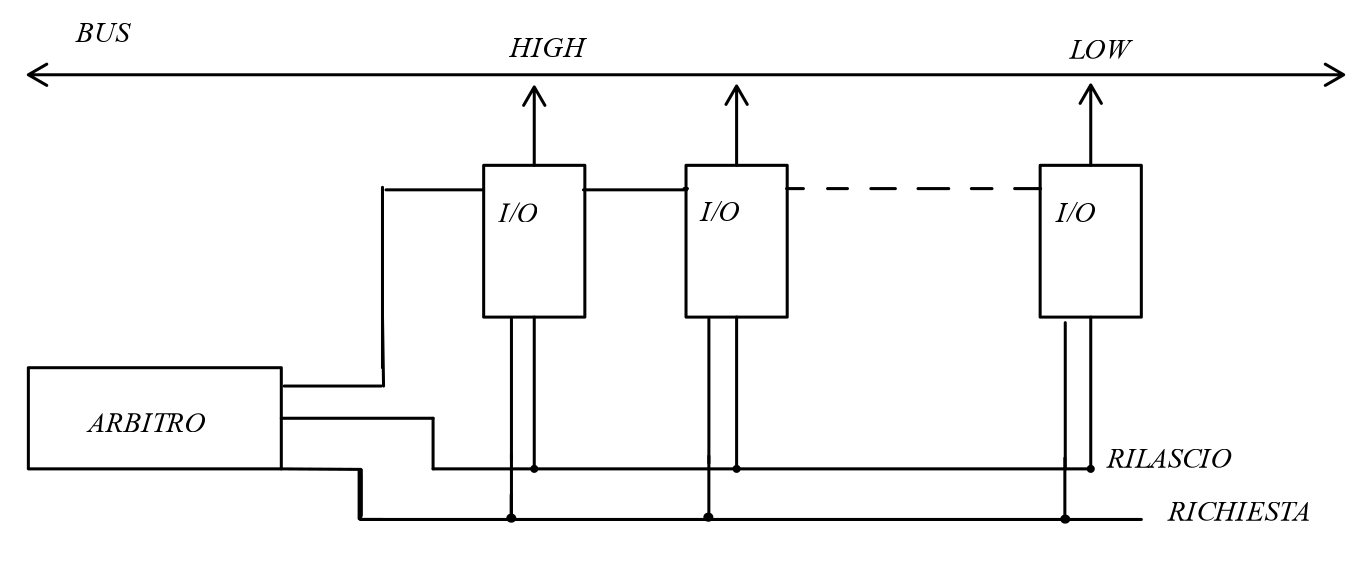
\includegraphics[scale=0.325]{img/daisy_chaining.png}
    \end{figure}
    \vspace*{10px}
\item \textbf{Richiesta Indipendente}: Una componente \textbf{arbitro} sceglie chi può o meno comunicare sul bus tra tutte le periferiche esterne:
\begin{figure}[htbp]
        \center
        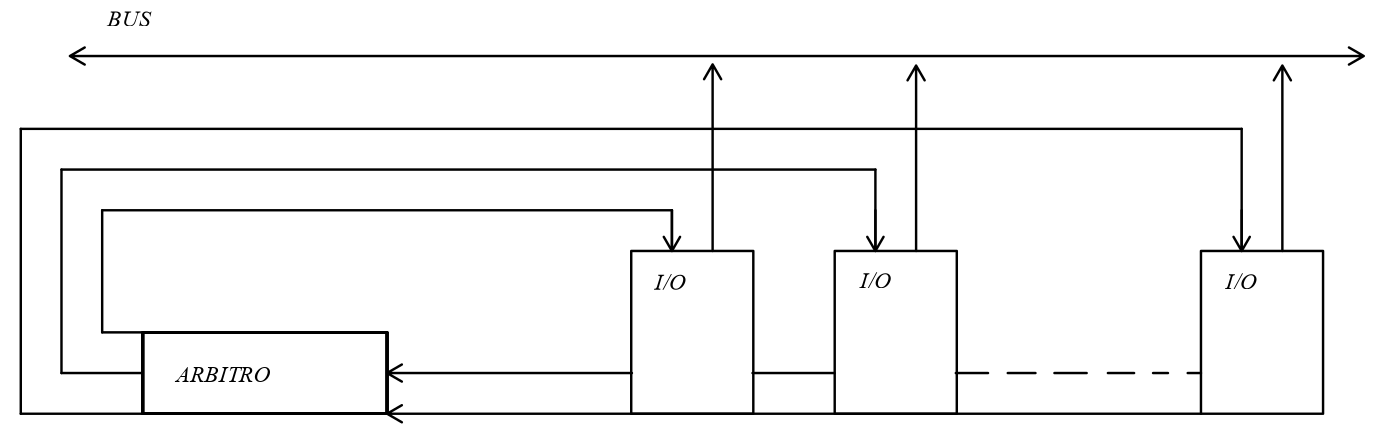
\includegraphics[scale=0.325]{img/richieste_indipendenti.png}
    \end{figure}
    \vspace*{10px}
\item \textbf{Token Passing}: Esiste una sorta di comunicazione "ad anello" su cui gira un \textbf{token}. Chi acquisisce il token ha il permesso di comunicare sul bus e al termine della loro operazione dovranno restituire il token:
\begin{figure}[htbp]
        \center
        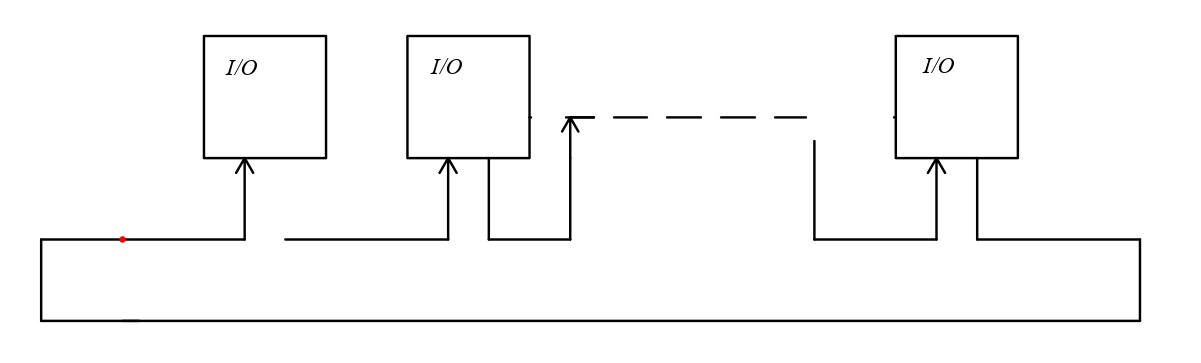
\includegraphics[scale=0.325]{img/token_passing.png}
    \end{figure}
\end{enumerate}

\vspace*{10px}

\newpage

\subsection{Meccanismi di Gestione Bus}

Una volta definita la composizione e gli arbitraggi del bus bisogna descrivere in che modo vengono inviati i dati ed i segnali grazie a specifici meccanismi.

\subsubsection{Memory Mapped I/O}

Immaginiamo di star lavorando con un architettura a 32 bit, \textbf{riserviamo} una quantità di questi \textbf{bit} in ogni indirizzo come \textbf{flag} che indichi se bisognerà o meno \textbf{dirottare} il contenuto verso la \textbf{memoria principale} o la \textbf{memoria} di qualche \textbf{periferica}.

\vspace*{10px}

    \begin{figure}[htbp]
        \center
        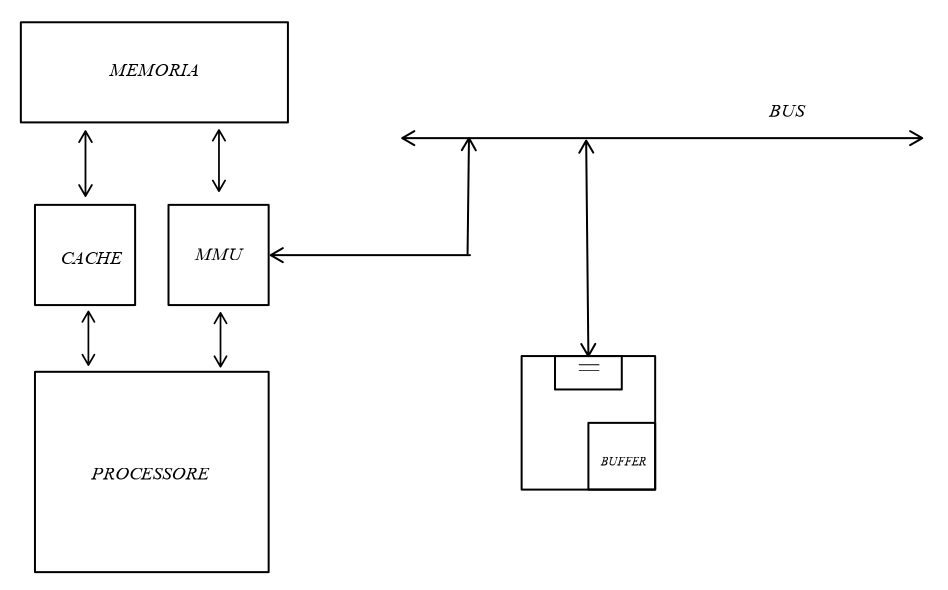
\includegraphics[scale=0.45]{img/memory_mapped_io.png}
    \end{figure}

\vspace*{10px}

L'unità che ci permette di effettuare questa scelta è la \textit{Memory Managment Unit} (\textbf{MMU}) che ha accesso sia alla memoria sia alle periferiche. Abbiamo quindi un modo per reindirizzare operazioni di load/store anche sul buffer delle periferiche.

\subsubsection{Interruzioni}

Un altro meccanismo fondamentale è quello della gestione delle interruzioni, ossia dei segnali che permettono la comunicazione tra periferiche e CPU. Immaginiamo che la CPU stia eseguendo questo loop:

\vspace*{10px}

\begin{lstlisting}[language = JavaScript]
    while (true){
        fetch
        decode
        execute
        memory
        write back
        interruzione?
    }
\end{lstlisting}

Questo ci permette di ottenere un segnale sul chi e perchè sia stata lanciata un interruzione (se è stata lanciata), in modo che la CPU possa agire di conseguenza.

\newpage

\subsection{Metodi di Query sullo Stato dell'I/O}

Assumiamo che la CPU abbia ordinato l'esecuzione di un istruzione ad una periferica. Come fa la CPU a sapere quando la periferica ha terminato l'operazione in questione? 

    \begin{figure}[htbp]
        \center
        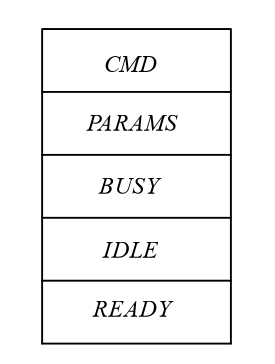
\includegraphics[scale=0.45]{img/buffer_periferica.png}
    \end{figure}


Presentiamo le due principali metodologie:

\begin{enumerate}
    \item \textbf{Programmed I/O}: Metodologia sincrona, la CPU effettua continue richieste alla periferica (nello specifico al campo \textit{ready} del suo buffer) per capire se l'operazione è conclusa. Elenchiamo nello specifico le fasi della CPU:
    \begin{enumerate}
        \item Controlla se la periferica è in \textit{idle}. Se lo è, assegna l'operazione (passando \textit{cmd} e \textit{params}).
        \item Controlla attivamente lo stato \textit{ready} della periferica in questione.
        \item Quando la periferica ha finito, acquisisce il risultato.
    \end{enumerate}

    \paragraph{Polling} E' possibile modificare questa attesa attiva grazie al fenomeno del polling, ossia una \textbf{frequenza} di \textbf{richiesta} al campo \textit{ready} del buffer della periferica. Questa frequenza va settata con cura, dato che richieste troppo frequenti si avvicinerebbero all'attesa attiva, mentre richieste poco frequenti causerebbero poca reattività. Questa metodologia causa quindi un rallentamento della CPU dato che si effettuerebbero molte operazioni inutili, ma si cerca di evitare la piena attesa attiva.

    \item \textbf{Interrupt Driven I/O}: Metodologia asincrona, la CPU carica l'istruzione alla periferica e attende non attivamente un segnale di terminazione da parte della periferica stessa. Illustriamo per step:
    \begin{enumerate}
        \item CPU legge l'\textit{idle} della periferica, se trova $1$ carica \textit{cmd} e \textit{params}.
        \item CPU riprende il suo ciclo standard, controllando ad ogni ciclo di clock se sono presenti segnali d'interruzione.
        \item Se dovessero incorrere delle interruzioni, la CPU salverebbe il corrente stato dell'operazione e analizzerebbe l'interruzione data.
    \end{enumerate}
    Questa metodologia ci permette di evitare il calcolo di un \textbf{polling} ottimale dato che sarà la periferica stessa a notificare il completamento dell'operazione grazie all'unità delle \textbf{interruzioni}.
\end{enumerate}

\newpage

\paragraph{System Bus} Notiamo che dopo le ultime modifiche è necessario che la memoria non sia collegata solo al processore. Di conseguenza viene posizionato un nuovo bus che permetta l'interazione diretta tra memoria e device esterni.

\begin{figure}[htbp]
        \center
        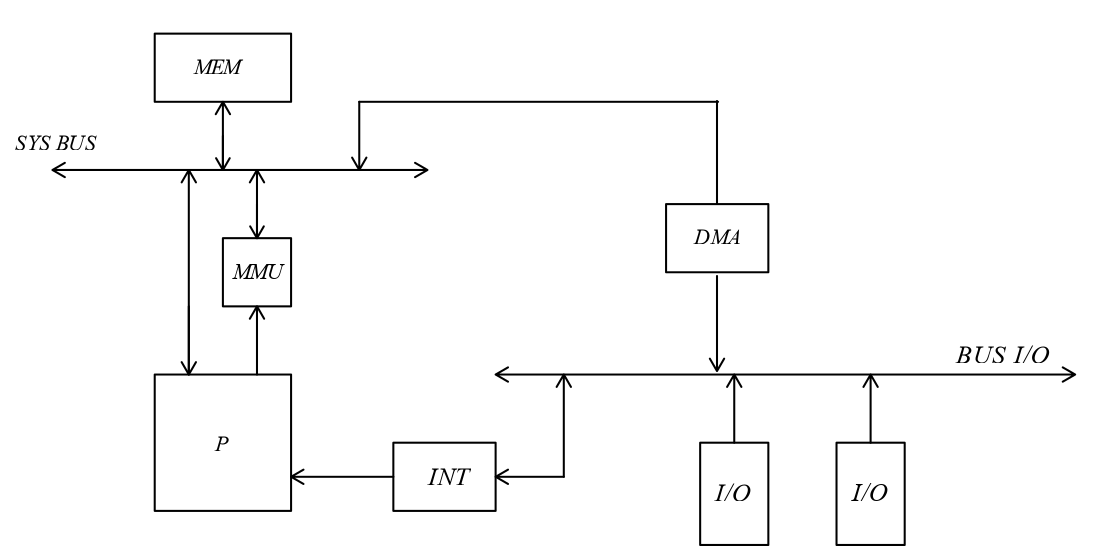
\includegraphics[scale=0.45]{img/bus_sys.png}
    \end{figure}

Il modulo \textit{Direct Memory Access} (\textbf{DMA}) permette l'interazione stabilita prima.

\paragraph{Priorità tra i due Bus} E' necessario stabilire a quale \textbf{bus} dare \textbf{priorità}. Sappiamo che le operazioni sui dispositivi di I/O sono molto più lente delle operazioni del processore, ma se ricevessimo un segnale d'interruzione risulterebbe molto probabile che il buffer del device che ha inviato l'interruzione è pieno. Di conseguenza, per prevenire perdite di dati dei buffer, si preferisce dare priorità al bus I/O.

\paragraph{DMA e Coerenza Cache} La coesistenza di \textbf{cache}, \textbf{buffer I/O} e \textbf{memoria} principale causata dal \textbf{DMA} può causare forte inconsistenza. Conosciamo infatti i meccanismi che permettono di tenere coerenti le linee di cache e le informazioni in memoria principale. In presenza del \textbf{DMA} si preferisce invalidare la cache, per evitare a monte di avere problemi con i meccanismi di coerenza citati prima.

\newpage

\section{Introduzione ai Sistemi Operativi}

Il sistema operativo è il software fondamentale per un calcolatore. Solitamente scritto in un linguaggio ad "alto" livello (es. C), si occupa della gestione del calcolatore (processi, I/O, memoria).

\begin{figure}[htbp]
        \center
        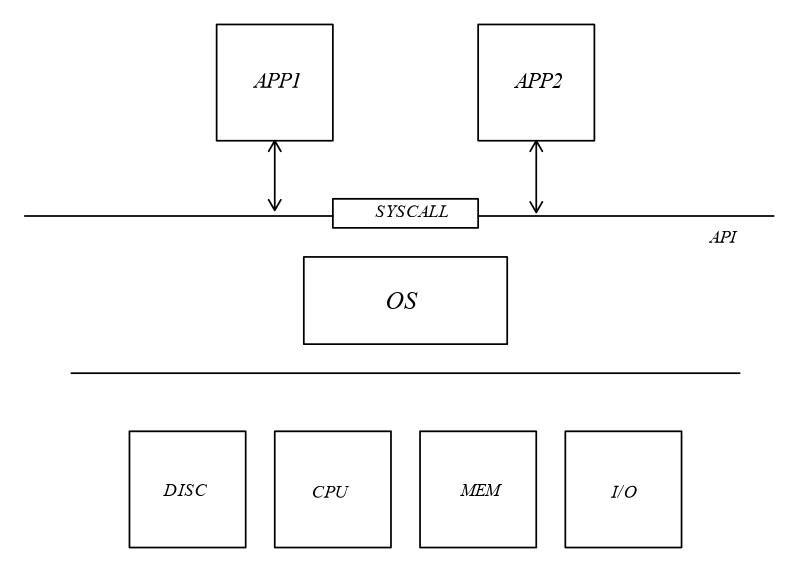
\includegraphics[scale=0.55]{img/os1.png}
    \end{figure}

\paragraph{Astrazioni del Sistema Operativo} Uno degli obiettivi del'OS è quello di rendere questi tre tipi di astrazione all'user:

\begin{enumerate}
    \item \textbf{Illusionist}: Il sistema operativo permette di immaginare spazi di memoria allocati in maniera contigua. Questo è più un concetto \textbf{logico} che fisico, infatti sarà lo stesso \textbf{OS} ad occuparsene a basso livello, astraendo l'user dalla gestione fisica della memoria.
    \item \textbf{Referee}: Il sistema operativo deve gestire le risorse condivise ed il settaggio delle proprietà di ciascun utente.
    \item \textbf{Glue}: Il sistema operativo mette a disposizione le librerie e le utilities necessarie alla coesistenza di CPU, memoria e disco.
\end{enumerate}

\paragraph{Proprietà Garantite dal Sistema Operativo} Per costruire l'astrazione, il sistema operativo deve garantire specifiche proprietà:

\begin{enumerate}
    \item \textbf{Affidabilità}
    \begin{enumerate}
        \item Disponibilità
    \end{enumerate}
    \item \textbf{Sicurezza}
    \item \textbf{Portabilità}
    \newpage
    \item \textbf{Performance}
    \begin{enumerate}
        \item Latenza
        \item Throughput (Tasso di produzione per unità di tempo)
        \item Overhead (Quanto lavoro aggiuntivo necessario alla resa dell'astrazione)
        \item Fairness (In presenza di più utenti, questi devono avere stesse possibilità di utilizzo delle risorse)
        \item Predictability (Possibilità di prevedere sommariamente il comportamento del sistema operativo in base al contesto)
    \end{enumerate}
\end{enumerate}

\begin{figure}[htbp]
        \center
        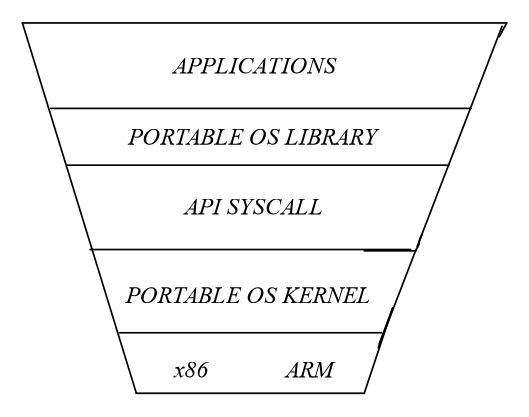
\includegraphics[scale=0.375]{img/stack_os.png}
    \end{figure}

\subsection{Struttura Kernel - Monolitica vs a Micro Kernel}

Esistono diversi modi per organizzare il nucleo di un sistema operativo, illustriamo le due metodologie agli antipodi:

\begin{enumerate}
    \item \textbf{Kernel Monolitico}: Tutto ciò che è a disposizione dell'OS è nel suo kernel, di conseguenza ogni modifica o aggiunta di funzionalità integrate comporta l'estensione del kernel stesso.
    \item \textbf{Micro Kernel}: L'effettivo kernel contiene solo pochissime funzionalità (come lo scheduling di attività o l'acquisizione dell'I/O), il resto delle attività vengono integrate come veri e propri processi.
\end{enumerate}

\subsection{Computazioni nel Tempo - (Batch, Spool, Time Sharing)}

Elenchiamo tre metodologie di gestione delle elaborazioni nei primi calcolatori:

\begin{enumerate}
    \item \textbf{Sistema Batch}: Assumiamo di avere una lista di \textit{jobs} da elaborare. \[ Batch = \{job_1,\:job_2, \:job_3\} \]
    Ognuno di questi \textit{job} si compone di parte CPU e parte I/O. Il sistema Batch è il più semplice, infatti eseguirà in maniera sequenziale i lavori.
    \item \textbf{Spool}: Con lo \textit{spool} si tenta di riempire i "vuoti" di elaborazione durante operazioni di I/O con calcoli con CPU del \textit{job} successivo che non risulti in nessun modo dipendente da quello prima.
    
    \newpage
    
    \item \textbf{Time Sharing}: La CPU eseguirà frazioni alternate di ogni \textit{job} in coda. Quando viene richiesto dell'I/O da un \textit{job} questo non sarà più contato in questa operazione di interleaving.
\end{enumerate}

\subsection{Protezione del Calcolatore}

Il sistema operativo deve occuparsi anche di meccanismi di \textbf{protezione} del calcolatore. Nello specifico, con protezione intendiamo dei meccanismi per cui ogni operazione sia legata a relativi \textbf{diritti} e \textbf{permessi}.

\vspace*{15px}

\subsubsection{Dual Mode - User/System}

Esistono vari ruoli in base al sistema operativo utilizzato che permettono o meno di eseguire determinate istruzioni. Mostriamo uno schema semplice basato su due ruoli, ossia \textbf{User} e \textbf{System}:

    \vspace*{10px}


\begin{enumerate}
    \item \textbf{User Mode}: L'user avrà \textbf{meno} \textbf{privilegi}, di conseguenza potrà eseguire meno istruzioni. Spesso l'user avrà modo di utilizzare funzioni "più ad alto livello" come ad esempio una \textit{fread} oppure una \textbf{syscall}, senza avere accesso direttamente alla routine di esecuzione effettuata dal sistema.
    \item \textbf{System Mode}: Il System avrà \textbf{più privilegi}, di conseguenza ha il permesso di eseguire più istruzioni. Una particolarità del "ruolo" System è quello di poter eseguire le routine invocate dalle \textbf{syscalls} degli user. Per questo l'invocazione di syscall causa uno switch di modalità, per fare in modo che la sua routine possa essere eseguita dal lato system.
\end{enumerate}

\vspace*{15px}

\subsubsection{Meccanismi Necessari alla Gestione del Dual Mode}

Per garantire una dual mode consistente l'OS deve prima fornire questi meccanismi:

\begin{enumerate}
    \item \textbf{Istruzioni Privilegiate}: Operazioni non eseguibili dall'user, sarà la \textit{CPSW} ad indicare se sarò o meno user. Degli esempi di istruzioni privilegiate:
    \begin{enumerate}
        \item Disabilitare le interruzioni.
        \item Scrivere manualmente nella \textit{CPSW}.
        \item Scrivere manualmente nel \textit{timer}.
    \end{enumerate}
    \newpage
    \item \textbf{Limitazione sugli Indirizzi di Memoria}: Si limitano gli indirizzi di memoria accessibili dall'user, rendendo visibile all'user solo una memoria virtuale che mappa su quella reale secondo degli schemi specifici, come ad esempio il \textit{Base \& Bound}.
    \begin{figure}[htbp]
    \center
    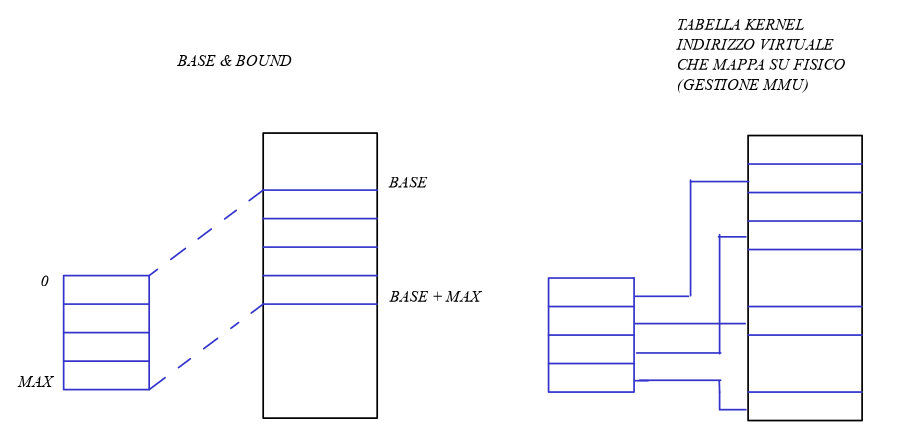
\includegraphics[scale=0.5]{img/ind_fisico_virtuale.png}
    \caption{Due esempi di limitazione e mapping di memoria virtuale su quella fisica.}
\end{figure}
\item \textbf{Timer}: Si definisce un modo per gestire interruzioni in caso di \textbf{overtime}, se un processo dovesse infatti "bloccarsi" avremmo un modo per gestire in maniera semiautomatica il suo overtime, interrompendolo nel caso in cui sia trascorso troppo tempo.
\item \textbf{Safe Ways per Switch Mode}: L'OS deve anche garantire metodologie \textbf{sicure} per lo \textbf{swap} tra le modalità user e system. In \textbf{ARM} una di queste metodologie è la \textit{SVC} (supervisor call), che funziona esattamente come una chiamata di funzione, ossia si aspetta i parametri nei registri $R_{0},R_{1},R_{2}\:\:...$ e nello specifico in $R_{7}$ si aspetta il codice della \textit{syscall} che si sta effettuando.

\begin{enumerate}
    \item \textbf{Esempio di una read}: Vediamo un esempio di syscall, ossia a cosa corrisponde effettuare una read:
    \vspace*{5px}
    \[ \boxed{read(file\_desc,\:buff,\:len)} \]
    \vspace*{5px}
\begin{lstlisting}[language = JavaScript]
    MOV R0, "file_desc"
    MOV R1, "buff"
    MOV R2, "len"
    MOV R7, "#CODICE_READ"
    SVC 0
\end{lstlisting}

Stiamo descrivendo in "pseudo ARM" le operazioni effettuate dall'invocazione della read, ossia una comune \textit{syscall}.

\end{enumerate}

In vari casi si effettuando degli \textbf{switch mode}, ad esempio \textbf{da user a supervisor} in casi come \textit{syscall}, \textit{interruzioni} o \textit{eccezioni}, mentre \textbf{da supervisor a user} in return dalle operazioni elencate prima, in \textit{creazioni di processi} e in \textit{upcall} (ossia se scatta il timer esegui una specifica operazione).

\end{enumerate}

\newpage

\subsection{Descrizione di un Processo}

Immaginiamo un processo che "nasce" da queste fasi:

\begin{enumerate}
    \item Un \textbf{programma} (codice sorgente) viene compilato.
    \item La \textbf{compilazione} produce un \textbf{eseguibile}.
    \item L'\textbf{eseguibile} viene lanciato, creando un \textbf{processo}.
    \begin{enumerate}
        \item Verrà allocata della memoria durante il lancio dell eseguibile, necessaria al corretto funzionamento del processo.
        \item Viene generato un \textbf{descrittore di processo} durante il lancio dell'eseguibile, per fare in modo che si possano mantenere dei \textbf{metadati} riguardanti il processo stesso.
    \end{enumerate}
    
\end{enumerate}

\subsubsection{Thread e Processi}

Assumendo che ogni \textbf{processo} abbia spazio d'indirizzamento indipendente dagli altri, possiamo descrivere le differenze con i \textbf{thread} che invece \textbf{condividono} tra loro memoria \textbf{dati} ed \textbf{istruzioni}. Dunque un processo sarà "composto" da più thread, che condivideranno lo spazio allocato per il processo "padre".

\subsubsection{PCB - Process Control Block}

Il \textbf{PCB} descrive un intero processo, portandosi dietro una serie di informazioni utili, elenchiamole:

\begin{enumerate}
    \item \textbf{PID}: ID del processo.
    \item \textbf{Stato Processo}: Corrente stato del processo (\textit{running}, \textit{new}, \textit{ready}, \textit{wait}, \textit{terminated}).
    \item \textbf{Registri CPU}: Stato architetturale, ossia contenuto dei registri della CPU durante l'esecuzione del processo.
    \item \textbf{Informazioni di Scheduling}: Priorità d'esecuzione assegnata al processo in questione.
    \item \textbf{Puntatore ai Thread}: Puntatore a tutti i thread che compongono il processo.
    \item \textbf{Informazioni su Memoria Allocata}: Informazioni sulla memoria allocata automaticamente che dovrà essere deallocata a tempo di terminazione del processo.
    \item \textbf{Informazioni su Risorse Allocate}: Informazioni su tutta la memoria allocata a supporto del funzionamento del processo (ad esempio descrittori di file).
\end{enumerate}

\newpage

\subsection{Descrizione Interruzioni}

Descriviamo tutti i meccanismi a supporto del funzionamento delle interruzioni:

\begin{enumerate}
    \item \textbf{Interrupt Vector}: La vera e propria interruzione sarà un semplice \textbf{codice} numerico. L'interrupt vector mappa a quel codice l'effettiva routine da eseguire nel caso venga rilevata l'interruzione in questione. Possiamo dunque definirla come zona di memoria che da contesto alle interruzioni in base al loro codice.
    \item \textbf{Kernel Interrupt Stack}: Nel momento in cui l'OS si accorge di un interruzione ha la necessità di salvare il corrente stato architetturale\footnote{Per stato architetturale s'intende il corrente contenuto dei registri.}. Tutti questi dati corrispondono però a dati di \textbf{sistema} e non di \textbf{user}, di conseguenza non possono essere pushati sullo stack regolare ma devono essere riposti nel \textbf{kernel stack}. In questo modo sappiamo dove il sistema dovrà riacquisire i dati dopo la completa elaborazione dell'interruzione.
    \item \textbf{Interrupt Masking}: Opzione di apertura/chiusura delle interruzioni, possiamo in questo modo disattivare la ricezione di interruzione durante specifiche fasi critiche.
    \item \textbf{Swap Mode Atomico}: Meccanismo di swap mode safe.
    \item \textbf{Ripartenza del Ciclo CPU Regolare}: Meccanismo di ripristino della routine standard del processore.
\end{enumerate}

\subsubsection{Handler di Interruzioni}

Gli \textbf{Handler} sono gestori di interruzioni ed hanno l'obiettivo di eseguire tutte le fasi necessarie all'elaborazione completa di un interruzione. Possono essere visti come \textbf{kernel threads}, si fermano solo quando hanno terminato di elaborare l'interruzione e hanno lo scopo di effettuare queste fasi:

\begin{enumerate}
    \item Salvare lo \textbf{stato} a tempo d'acquisizione dell'interruzione.
    \item \textbf{Trattare l'evento} in base alla \textbf{specifica interruzione} ricevuta.
    \item \textbf{Interagire} con lo schedulatore per dare \textbf{priorità} all'evento legato 
    
    all'elaborazione dell'interruzione.
\end{enumerate}

Dopo la sua esecuzione vanno restabiliti: \textbf{stato precedente}, \textbf{program stack}, \textbf{parola di stato} e \textbf{modalità utente}, ripristinando anche il funzionamento delle interruzioni.

\paragraph{Interruzioni in ARM} In architettura \textbf{ARM} quando il processore coglie un interruzione a fine del suo ciclo standard, va nell'unità \textbf{INT}, che ha una "propria memory mapped I/O", ricavando così le informazioni sul chi e sul perchè sia stata sollevata l'interruzione in questione.

\newpage

\subsection{Esempi d'Implementazione su Architettura ARM}

Mostriamo come meccanismi generici dei sistemi operativi vengano implementati su ARM.

\subsubsection{CPSR ed Interrupt Masking}

Nel registro \textbf{CPSR} (Current Program Status Register) sono presenti delle informazioni riguardanti le interruzioni, infatti:

\begin{enumerate}
    \item \textbf{Bit I (Interrupt)}: Questo bit, solitamente settato a $0$ può essere cambiato in $1$ effettuando così un mask. Questo ci permetterebbe temporaneamente di ignorare tutte le interruzioni.
    \item \textbf{Bit F (Fast Interrupt)}: Funziona allo stesso modo, a differenza del normale Interrupt il Fast Interrupt salva parte dello stato architetturale automaticamente in specifici registri ombra.
\end{enumerate}

Un bit tra quelli del \textbf{CPSR} è dedicato anche al \textbf{Thumb Arm}, settando ad $1$ la \textbf{flag} si ha infatti la possibilità di \textbf{switchare} in direzione di ARM su istruzioni di dimensione dimezzata.

\subsubsection{Modalità di Esecuzione}

In ARM esistono \textbf{diverse} modalità di esecuzione, elenchiamole:

\vspace*{5px}

\begin{center}
    \begin{tabular}{|c|c|}
    \hline
    MODE & CODICE NELLA CPSR  \\
    \hline
    User & $10000$ \\
    \hline
    Supervisor & $10011$ \\
    \hline
    Abort & $10111$ \\
    \hline
    Undefined (Reserved) & $11011$ \\
    \hline
    Interrupt & $10010$ \\
    \hline
    Fast Interrupt & $10001$ \\
    \hline
    \end{tabular}
\end{center}

\vspace*{5px}


Nello specifico queste modalità avranno un vettore con locazioni contenenti ciascuna la routine da eseguire in caso di switch di modalità.

\vspace*{5px}

\begin{center}
        \begin{tabular}{ |c| } %|c|c|c|%
         \hline
         Reset \\
         \hline
         Undefined \\ 
         \hline
         Supervisor Call \\
         \hline
         Prefetch Abort \\
         \hline
         Data Abort \\
         \hline
         Reserved \\
         \hline
         Interruption \\
         \hline
         Fast Interruption \\
         \hline
        \end{tabular}
    \end{center}

\vspace*{5px}

In questo vettore \textbf{non saranno presenti} i puntatori alle routine delle modalità, infatti saranno presenti \textbf{direttamente} le routine da eseguire sotto forma di istruzioni ASM.

\newpage

\paragraph{Fasi di Swap Mode} Descriviamo in dettagli tutti i passi necessari ad uno scambio di modalità:

\begin{enumerate}
    \item In \textbf{Banked LR} salvo in corrente \textbf{PC}.
    \item In \textbf{SPSR} (Banked CPSR) salvo la corrente \textbf{CPSR}.
    \item Cambio i $5$ bit che definivano la mia corrente proprietà nella \textbf{CPSR}.
    \item Cambio \textbf{Reg} in \textbf{Reg Banked}.
    \item Disabilito le \textbf{Interrupt}.
    \item In \textbf{PC} metto il codice del \textbf{mode} verso cui voglio switchare
\end{enumerate}

Ognuna di queste fasi viene eseguita in maniera \textbf{atomica} per mantenere consistenza.

\subsubsection{Banked Registers}

In ARM alcuni registri si definiscono \textbf{banked} perchè preservati in maniera automatica, anche durante lo swap di modalità.
\begin{enumerate}
    \item \textbf{Int, SVC, Abort, Undefined}: Queste quattro modalità hanno come banked registers $SP$ ed $LR$.
    \item \textbf{Fast Int}: Ha come banked registers $R8 \: - \: R12$, $SP$ ed $LR$.
\end{enumerate}

\subsection{System Calls}

\vspace*{5px}

Definiamo le \textbf{SYSCALLS}, ossia una sorta di chiamata di procedura ma in direzione del sistema operativo, \textbf{caratterizzata} da uno \textbf{swap di modalità} durante la sua esecuzione.

Il flusso di una syscall è così definito (esempio su architettura ARM):

\vspace*{5px}

\begin{enumerate}
    \item L'\textbf{User} effettua la chiamata al sistema.
    \item Si \textbf{switcha} verso l'\textbf{SVC}.
    \item Si \textbf{settano} i \textbf{parametri} forniti dall'\textbf{user} in maniera tale da renderli \textbf{leggibili} anche in \textbf{modalità system} (scambi con i banked registers oppure effettuando delle pop dal kernel stack).
    \item Si chiama la \textbf{routine della syscall} indirizzandosi sulla tabella che contiene le routine stesse grazie al \textbf{codice assegnato} alla corrente syscall.
\end{enumerate}

Queste operazioni, dallo switch di modalità in poi, sono eseguite dal \textbf{Call Handler}.

\vspace*{10px}

Mostriamo nel successivo sottocapitolo un esempio di implementazione in ASM ARM v7 di Call Handler.

\newpage

\subsubsection{Call Handler in ASM ARM v7}

Mostriamo una possibile implementazione di \textbf{Call Handler} commentandola successivamente.

\vspace*{5px}


\begin{lstlisting}[language = JavaScript]
    STMFD SP!, {R0-R12,LR}
    ADR R8, BASE_SYS_CALL_TABLE
    @CHECK
    LDR PC, [R8,R7,LSL #2]
    LDMFD SP!, {@PARAMETRI PREC.}
    MOVS PC, LR
\end{lstlisting}

\begin{enumerate}
    \item Store multipla dei registri e del link register per \textbf{salvare} lo stato \textbf{architetturale corrente}.
    \item Si mette in r8 la $BASE\_SYS\_CALL\_TABLE$ (base della tabella delle syscalls) grazie all'istruzione $ADR$.
    \item Si cambia il $PC$ grazie ad una load nella \textbf{tabella delle syscall} con \textbf{base} 
    
    d'indirizzamento in $R8$ e con il \textbf{codice di syscall} in $R7$, ricordando di star lavorando su indirizzi che vanno di quattro in quattro (caratteristica dell'ARM v7).
    \item \textbf{Restore} dello \textbf{stato architetturale} pre-call.
    \item Si \textbf{ristabilisce} il vecchio \textbf{Program Counter} per \textbf{ritornare} a chi ha invocato la syscall.
\end{enumerate}

\subsection{Upcalls - Segnali}

In user mode abbiamo la possibilità di registrare un \textbf{handler} che verrà invocato dal \textbf{kernel} a tempo dell'occorrenza di uno specifico \textbf{evento}. Il concetto di \textbf{up} deriva dal fatto che sto definendo qualcosa a livello \textbf{user} che verrà eseguito dal \textbf{kernel} quando necessario. Elenchiamo altre caratteristiche vantaggiose delle upcalls:

\begin{enumerate}
    \item Gestiscono lo stack \textbf{user-space} in \textbf{maniera distaccata} dal resto delle informazioni.
    \item Hanno meccanismi di \textbf{auto salvataggio} dei \textbf{registri}.
    \item Permettono il \textbf{masking} degli \textbf{altri segnali} durante l'esecuzione di un handler.
\end{enumerate}

\subsection{Kernel Boot}

Descriviamo cosa accade all'accensione di un calcolatore:

\begin{enumerate}
    \item La \textbf{CPU} accede ad una locazione di una memoria ROM/EEPROM facendo in modo che il \textbf{BIOS} possa caricare il \textit{first stage bootloader}.
    \item Questa \textbf{prima forma} di \textbf{bootloader} inizializza il controllo della memoria, qualche dispositivo di I/O e \textbf{carica} il \textit{second stage bootloader}.

\newpage

    \item Questa \textbf{seconda forma} di \textbf{bootloader} si occupa del caricamento del \textbf{kernel} del sistema operativo e della \textbf{root} del file system, lasciando infine il controllo al kernel.

\end{enumerate}

\subsection{Sommario Specifiche Hardware Necessarie all'OS}

Possiamo dunque riassumere tutti i minimi meccanismi necessari alla composizione di un sistema operativo consistente:

\begin{enumerate}
    \item \textbf{Livelli di Privilegio}: E' necessaria l'esistenza di \textbf{almeno} due livelli di privilegio (user/system) anche se abbiamo visto che in ARM ne sono presenti diversi (SVC, Abort, User, Interrupt...)
    \item \textbf{Istruzioni Privilegiate}: Istruzioni eseguibili \textbf{solo se} \textbf{non} siamo in \textbf{modalità user} per garantire sicurezza.
    \item \textbf{Traduzione Indirizzi Memoria}: Meccanismo di map di \textbf{indirizzi} \textbf{virtuali} disponibili a reali \textbf{indirizzi} di memoria \textbf{fisici}.
    \item \textbf{Eccezioni}: Routine eseguite in caso di \textbf{violazione di privilegi}.
    \item \textbf{Interruzioni}: Meccanismo di interruzioni che permetta la \textbf{comunicazione} tra \textbf{device} e \textbf{CPU}.
    \item \textbf{Mask di Interruzioni}: Meccanismo che ci permetta di disattivare le interruzioni in fasi critiche.
    \item \textbf{Syscalls}: Interfaccia tra \textbf{utente} e \textbf{macchina} tramite invocazione di operazioni "standard", dunque possibilità di esecuzione di azioni privilegiate da un programma user.
    \item \textbf{Boot}: Routine di avvio della macchina.
    \item \textbf{Operazioni Atomiche su Memoria}: Operazioni in memoria il cui utilizzo \textbf{garantisce consistenza} anche in contesti multithread.
    \item \textbf{Virtualizzazione}: Gestione di \textbf{hypervisors} che permettano di creare \textbf{diversi ambienti virtuali} anche sulla stessa macchina fisica. 
\end{enumerate}

\newpage

\section{Interfaccia di Programmazione di Applicazioni di un OS}

Un sistema operativo deve fornire un interfaccia che permetta di:

\begin{enumerate}
    \item Creare \textbf{processi} e gestirli.
    \item Gestire l'\textbf{I/O} fornendo operazioni di apertura, chiusura, scrittura e lettura.
    \item Gestire la \textbf{comunicazione} tra \textbf{processi} (IPC).
\end{enumerate}

In questo capitolo descriveremo quindi la gestione di questi meccanismi fondamentali che dei sistemi operativi devono offrire.

\subsection{Gestione Processi - (Fork, Exec, Wait, Sleep, Exit)}

I processi vengono creati e differenziati grazie a due specifiche \textbf{syscalls}:

\begin{enumerate}
    \item \textbf{Fork}: Crea un processo clone al padre che sta effettuando la chiamata alla fork. Si effettua una \textbf{copia}
    on demand del primo PCB (Process Control Block). Non viene dunque copiato tutto il blocco descrittore del padre a priori, ma verrà utilizzato
    come riferimento nel caso in cui sia necessario. Si genera dunque un nuovo \textbf{PID}, ossia id del processo. Non è assicurato che la syscall sia un 
    successo, di conseguenza se qualcosa dovesse far fallire la syscall verrebbe inserito $-1$ in \textit{errno}.

    \vspace*{10px}
\begin{lstlisting}[language = C]
    pid_t pid = fork(); // Valore > 0 se padre, == 0 se figlio, -1 se fallisce, in modo da distinguere facilmente i processi
    if (pid > 0) {
        printf("Sono il padre");
    } else if (pid == 0) {
        printf("Sono il figlio");
    } else {
        perror("fork failed");}
    \end{lstlisting}    

    \item \textbf{Exec}: Differenzia il codice presente nel \textbf{PCB} di riferimento. In questo modo il processo figlio avrà modo di eseguire
    istruzioni diverse dal padre. Esistono due tipi di exec, la \textbf{exec list (l)} ed \textbf{exec vector (v)} in base a come si aspettano i parametri
    che gli stiamo fornendo. Elenchiamo tutte le caratteristiche di questa syscall:
    \paragraph{Passi effettuati da una Exec}
    \begin{enumerate}
        \item \textbf{Rimpiazzamento} del \textbf{codice} del \textbf{padre} nel PCB corrente.
        \item Se ha successo, non ritorna.
        \item \textbf{Mantiene PID e PCB} assegnati durante la fork.
        \item \textbf{Resetta} segnali (\textbf{upcalls}) pendenti.
        \item Mantiene le risorse assegnate.
    \end{enumerate}

    
\newpage

\item \textbf{Wait}: Se un processo padre, dopo averlo creato volesse l'esito del figlio allora dovrebbe effettuare l'operazione di \textbf{wait (attesa)}
su quest'ultimo. Se un processo padre effettuasse la exit prima della terminazione del figlio allora quest'ultimo si definirebbe
\textbf{processo zombie}. Il \textbf{sistema operativo} ha però la responsabilità di occuparsi anche di questi casi limite, infatti assegnerà al processo zombie
un nuovo processo padre, ossia \textit{init}, che dovrà occuparsi della \textbf{deallocazione} delle \textbf{risorse} utilizzate per la descrizione
del processo figlio.

\item \textbf{Sleep}: Questa syscall permette allo scheduler di effettuare degli \textbf{swap} tra processi eseguiti in maniera "esplicita". Ricordiamo che infatti
lo scheduler non è un vero e proprio componente ma più un automa che ha una quantità di stati a disposizione ed effettua transizioni tra stati
in base agli input forniti. Se infatti un $processo1$ dovesse invocare la $sleep$ allora verrebbe \textbf{rischedulato} un \textbf{processo pronto} all'esecuzione.
    
\item \textbf{Exit}: Se un processo figlio chiama la exit, quest'ultimo termina chiudendo tutte le risorse ad esso allocate, e viene salvato un codice di uscita
passato ad exit come argomento. Il processo figlio sarà zombie fino a quando il processo padre non acquisirà il codice dato in argomento dalla exit
e salvato dal kernel. L'acquisizione da parte del padre di questo codice è effettuata con una \textit{wait} oppure una \textit{waidpid}.

\end{enumerate}

\subsection{Comunicazioni tra Processi - (Pipe)}

A differenza dei thread che hanno la possibilità di condividere memoria e dunque di comunicare tramite essa, i \textbf{processi} hanno \textbf{spazi d'indirizzamento dedicati}. Di conseguenza risulta necessario definire dei meccanismi che permettano a due (o più) processi di \textbf{comunicare} tra loro. In Unix questo viene
gestito in maniera "regolare" grazie alla gestione di ogni cosa come se fosse un file. Questo ci permette di aprire "file speciali" con specifici \textbf{descrittori}
di file in lettura e scrittura che gestiscono la comunicazione tra processi. Nello specifico in Unix questa gestione "a file" (ossia gestione dell'I/O) segue questi specifici principi:

\begin{enumerate}
    \item \textbf{Tutto} è visto come un \textbf{file}.
    \item Si segue un principio di \textbf{uniformità}, basando ogni operazione di I/O su open, read, write e close.
    \item Tutto il sistema è detto \textbf{Orientato al Byte}, ossia si stabilisce un interpretazione al byte delle informazioni lette.
    \item Le read/write saranno \textbf{Kernel Buffered}, sarà dunque il kernel ad occuparsi del buffer utilizzato durante queste syscalls.
    \item Alla fine va effettuata sempre una \textbf{close}, che permette il \textbf{flush} delle operazioni eseguite.
\end{enumerate}

Ma perchè questo nel capitolo dedicato alla comunicazione interprocesso? Perchè in qualche modo anche questa in Unix è gestita ad apertura e chiusura
di file e relativi descrittori in lettura/scrittura. Elenchiamo le caratteristiche nella pagina successiva.

\newpage

\paragraph{Descrittori in Lettura/Scrittura e Chiusura Duale} Ogni "file di comunicazione" aperto avrà queste caratteristiche:

\begin{enumerate}
    \item \textbf{Buffer in Lettura}: Buffer che permette la lettura in un solo verso tra due processi.
    \item \textbf{Buffer in Scrittura}: Buffer che permette la scrittura in un solo verso tra due processi.
    \item \textbf{Chiusura Duale}: Fino a quando sarà possibile scrivere in un buffer sarà vietata la sua chiusura
\end{enumerate}

Mostriamo pseudocodice C dell'utilizzo della syscall pipe e dei buffer che genera:

\vspace*{10px}
\begin{lstlisting}[language = C]
    int fd[2]; // fd[0] parte lettura, fd[1] parte scrittura
    if (pipe(fd) == -1) { // Creazione della pipe
        perror("pipe failed");
        exit(1);
    }
    /* Grazie alla gestione dei PID non scriveremo codice diverso
    per ciascun processo, infatti eseguiremo istruzioni diverse in base al valore del PID */
    pid = fork();
    if (pid > 0) { // Processo padre
        close(fd[0]); // Chiude il lato di lettura
        write(fd[1], "Hello, child!", 14);
        close(fd[1]); // Chiude il lato di scrittura
    } else if (pid == 0) { // Processo figlio
        close(fd[1]); // Chiude il lato di scrittura
        read(fd[0], buffer, sizeof(buffer));
        printf("Child received: %s\n", buffer);
        close(fd[0]); // Chiude il lato di lettura
    } else {
        perror("fork failed");
        exit(1);
    }
\end{lstlisting}

Questo meccanismo di comunicazione è unidirezionale (padre scrive e figlio legge), di conseguenza se volessimo gestire la comunicazione in entrambi i versi
risulterebbe necessario creare una pipe gestita in maniera speculare ma in verso opposto di comunicazione.

\newpage

\subsection{Gestione Threads}

Uno degli obiettivi di un Sistema Operativo è quello di implementare l'MTAO (Multiple Things at Once) e di coordinare queste moltepici operazioni
eseguite in contemporanea. Fino ad ora avevamo infatti visto solo dei processi, la cui struttura era indipendente e "monolitica", ciascuno aveva
a disposizione il proprio spazio d'indirizzamento (testo, dati, stack, ...) ma risulterebbe comodo al sistema operativo avere anche unità più
dinamiche e schedulabili in base alle necessità.

\paragraph{Definizione e Motivazioni di Utilizzo Threads} Flusso di controllo schedulabile, ossia che può essere mandato in esecuzione. Può essere visto come una "parte" di programma
che ha vita propria e che può essere mandata in esecuzione. Motivazioni:

\begin{enumerate}
    \item \textbf{Strutturazione}: Un programma può essere visto come composizione di tanti moduli indipendenti ma che agiscono sulle stesse risorse.
    \item \textbf{Reattività}: Dei calcolatori potrebbero avere la necessità di essere molto reattivi, l'utilizzo dei threads potrebbe ad esempio aiutare
    nel caso di polling su dispositivi I/O, fornendo così un approccio alternativo a quello tradizionale delle interruzioni.
    \item \textbf{Multicore}: La gestione a moduli separati permette un reale utilizzo delle risorse offerte da architetture multicore.
    \item \textbf{Performance}: La gestione parallela consistente permette il raggiungimento di ottime performance rispetto ad una esecuzione esclusivamente basata sull'interleaving.
\end{enumerate}

Ogni processo può essere dunque composto da più thread i quali ereditano i diritti del processo che li "possiede".

\paragraph{User/Kernel Thread} Un punto da analizzare è quello sulla visibilità del kernel sui threads. Un \textbf{User Thread} risulterebbe invisibile
alla schedulazione reale del kernel, verrebbe dunque del tutto gestito dal processo che lo possiede. Questo va ad intaccare il concetto di "modularità"
proprio perchè sarà impossibile per il kernel schedulare l'esecuzione di quel thread, potra a massimo infatti mandare in esecuzione il processo che lo contiene.
Per queste motivazioni si preferiscono attualmente strategie basate sui \textbf{Kernel Threads}, creano un po' più di overhead ma sono del tutto visibili
dal kernel che avrà modo di schedularli.

\vspace*{5px}

\begin{center}
    \begin{tabular}{ c|c|c } 
    Stato & Dov'è il TCB & Dove sono i Registri del Thread \\ 
        \hline
    INIT & ? & TCB \\ 
    READY & Lista Ready & TCB \\
    RUN & Lista Exec & Registri Processore \\ 
    WAIT & TCB(wait) & TCB \\ 
    END & ? & TCB \\ 

    \hline
    \end{tabular}
    \end{center}

\vspace*{5px}

Ogni thread avrà dunque uno \textbf{stack privato}, il codice e l'heap \textbf{condivisi}, mentre le variabili dipenderanno dal modo in cui vengono
dichiarate (se thread local o meno).

\newpage

\subsubsection{Schedulazione e Potenziale Inconsistenza}

Dato che abbiamo definito i threads come flussi schedulabili che hanno accesso allo stesso spazio d'indirizzamento è necessario definire "formalmente"
cosa significhi la parola schedulazione.

\begin{figure}[htbp]
    \center
    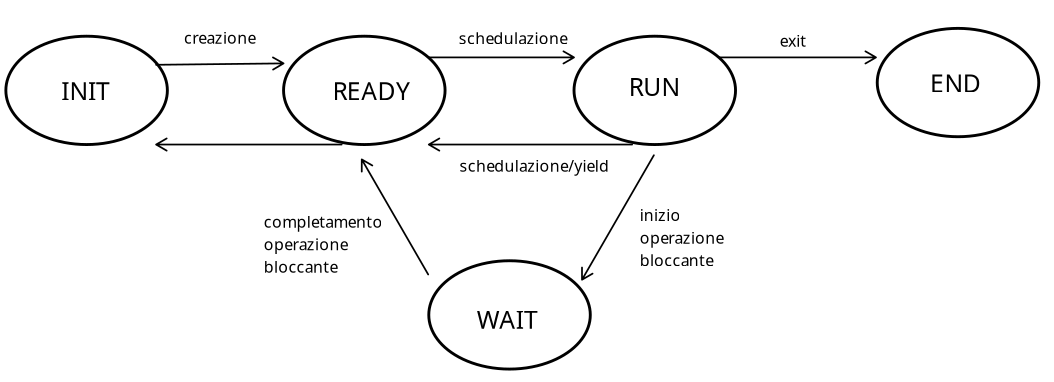
\includegraphics[scale=0.325]{img/automa_schedulatore.png}
    \caption{Automa della schedulazione.}
\end{figure}

Lo \textbf{schedulatore} non è un vero e proprio componente, ma più una reazione all'input rispetto allo stato in cui si trova un thread. E' quindi rappresentato
meglio da una serie di routine da eseguire in specifici eventi che accadono. E' necessario dunque che il codice scritto sia adatto ad un contesto multithread, per
fare in modo che sia corretto in ogni tipo di schedulazione. Risulta infatti impossibile prevedere in che ordine saranno schedulati i threads. 

\paragraph{Thread Control Block (TCB) e Transizioni di Stato} Le varie funzioni eseguibili provocheranno cambi di valori all'interno dei TCB, elenchiamo ad esempio alcune operazioni effettuate durante
una thrdCreate:

\begin{enumerate}
    \item Si crea il TCB del nuovo thread.
    \item Si settano il program counter del thread e tutto il suo stato architetturale in modo tale che quest'ultimo possa eseguire il suo runnable\footnote{Runnable, in Java è la funzione eseguita da un thread, usato come sinonimo di "funzione del thread".}. 
    In realtà il thread non esegue direttamente il runnable, ma una funzione wrapper detta \textbf{stub} che chiamerà il runnable,
    questo perchè è necessario coprire anche il caso in cui il runnable ritorni invece di effettuare una $thread\_exit$. Senza questo passo in più
    il runnable ritornerebbe ad una qualsiasi posizione sul top dello stack. In questo modo invece il runnable ritornerà allo stub e questo eseguirà la $thread\_exit$.
    \item Si setta lo stato nel TCB a ready (schedulazione).
    \item Si segnala a chi è in coda ready che l'esecuzione della create è finita.
    \item Si ritorna.
\end{enumerate} 

\newpage

\subsubsection{Yield/Interruzione di Thread}

Definiamo i modi in cui i thread passano ad uno stato di WAIT grazie ad una deschedulazione.

\begin{enumerate}
    \item \textbf{Yield}: Deschedulazione volontaria, gestita in modi diversi dal tipo di thread:
    \begin{enumerate}
        \item \textbf{User Thread Yield}: Viene effettuata la deschedulazione volontaria seguendo questi passi:
        \begin{enumerate}
            \item Salvataggio \textbf{stato architetturale} nel TCB (nello specifico nell'area registri).
            \item Si effettua lo switch verso un nuovo thread, questo comporta un \textbf{passaggio} ad un \textbf{nuovo stack}, che tecnicamente
            corrisponde a \textbf{copiare} nei registri l'\textbf{area registri} contenuta nel TCB del thread che stiamo schedulando. Questa fase
            è definita come commutazione di contesto e comporta un costo in tempo per il calcolatore.
            \item Si effettua il return.
        \end{enumerate}
        \item \textbf{Kernel Thread Yield}: Viene effettuata la deschedulazione volontaria seguendo questi passi:
        \begin{enumerate}
            \item Si effettuano gli stessi passi di un User Level Thread tranne per il fatto che il return corrisponderà esattamente
            ad una modifica al program counter.
        \end{enumerate}
    \end{enumerate}
    \item \textbf{Interrupt}: Assumiamo che un thread possa essere interrotto dall'I/O oppure da un timer, esistono due modalità di "risposta":
    \begin{enumerate}
        \item \textbf{Modalità Semplice}: Si seguono questi step:
        \begin{enumerate}
            \item L'Interrupt Handler salva i registri nel Kernel Stack.
            \item Si effettua lo switch di thread.
            \item Dopo l'esecuzione si ripristinano i registri precedentemente pushati nel Kernel Stack.
        \end{enumerate}
        \item \textbf{Modalità Veloce}: Si seguono questi step:
        \begin{enumerate}
            \item L'Interrupt Handler salva i registri correnti nel relativo TCB del thread interrotto.
            \item L'Interrupt Handler carica i registri dal TCB del thread che vuole far partire.
        \end{enumerate}
    \end{enumerate}
\end{enumerate}

In conclusione possiamo dunque affermare che la commutazione comporta un costo e che un approccio multithread è quello più adatto ad architetture multicore.

\newpage

\section{Sincronizzazioni}

La gestione multithread del flusso di un programma complica la situazione, dato che risulta necessario garantire consistenza dei risultati qualsiasi sia
la schedulazione dei thread in gioco. Elenchiamo dunque tutti i punti fondamentali della sincronizzazione e le problematiche che bisogna gestire:

\begin{enumerate}
    \item \textbf{Race Condition}: Condizione nella quale l'output del programma risulta dipendente dalla velocità relativa e dai tempi dei threads. Questa è la
    classica condizione che causa inconsistenza in contesti multithread, dato che si otterranno risultati completamente diversi ciascuna esecuzione del programma,
    data la completa dipendenza dal tipo di schedulazione.
    \item \textbf{Mutua Esclusione}: Definiamo delle sezioni critiche in cui solo un thread ha il permesso di operare. Spesso questo meccanismo è utilizzato
    durante operazioni su risorse condivise tra threads. Bisogna ricordare anche però che questa gestione causa un vero e proprio blocco delle esecuzioni in parallelo, 
    di conseguenza risulta necessario operare in mutua esclusione solo su brevi operazioni necessarie.
    \item \textbf{Lock}: Meccanismo che garantisce di operare in mutua esclusione. Le operazioni effettuate solitamente sono di lock/unlock.
    \item \textbf{Correttezza}: Garanzia che l'esecuzione rimarrà consistente a prescindere dal tipo di schedulazione effettuata durante quella specifica
    esecuzione.
    \item \textbf{Fairness}: Tutti i threads devono avere le stesse possibilità sull'utilizzo della CPU.
    \item \textbf{Conclusione Programma}: Non devono esistere possibili condizioni di stallo e/o di starvation, condizione per cui non è presente un
    effettivo stallo ma un task non viene schedulato mai data una cattiva gestione delle priorità.
\end{enumerate}

Analizziamo dunque tutti i tipi di \textbf{meccanismi di sincronizzazione} tra threads nelle pagine successive.

\subsection{Spinlock}

Meccanismo di attesa attiva sullo stato locked di un mutex. A differenza dei meccanismi che vedremo successivamente
non cerca di deschedulare un thread per poi risvegliarlo successivamente, ma lo lascia attendere attivamente in modo tale che
quando la risorsa sarà liberata quest'ultimo potrà accedervi. In specifici contesti questo approccio risulta più economico in termini di tempo
dato che non comporta nessuna commutazione di contesto. Spesso questo è implementabile in maniera abbastanza semplice dato che diverse architetture offrono
istruzioni specifiche che causano dei comportamenti corrispondenti ad una spinlock.

\vspace*{5px}

\begin{lstlisting}[language = C]
    EXCH r0, [r1, r2]
\end{lstlisting}

\vspace*{-8px}

Semanticamente corrisponde a $ MEM[r1+r2] \rightleftarrows r0 $, settando dei valori di default di $0$ chiuso ed $1$ aperto se cicliamo su questa istruzione abbiamo implementato uno spinlock in ARM.

\newpage

\subsection{Lock}

Il lock è un oggetto condiviso tra i vari thread, ciascuno di essi può effettuare due operazioni:

\begin{enumerate}
    \item \textbf{Lock/Acquire}: Si attende che il lock sia aperto e lo si acquisisce.
    \item \textbf{Unlock/Release}: Si apre il lock e si sbloccano potenziali threads in attesa.
\end{enumerate}

\begin{figure}[htbp]
    \center
    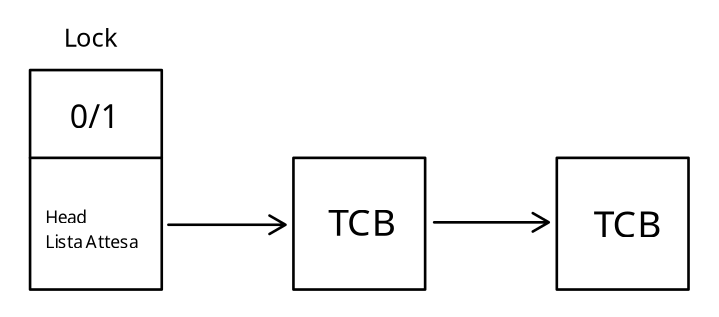
\includegraphics[scale=0.325]{img/rappresentazione_lock.png}
\end{figure}

Il release dunque se dovesse trovare almeno un elemento nella lista allora non setterebbe il lock a $0$ ma lascerebbe il controllo direttamente
al prossimo thread.

\paragraph{Proprietà Garantite dai Lock} Utilizzando questo meccanismo riusciamo a garantire queste proprietà:

\begin{enumerate}
    \item \textbf{Safety}: Viene eseguita una sola attività concorrente alla volta.
    \item \textbf{Liveness}: Se il lock è aperto l'acquire lo prende, mentre se chi ha il lock effettua la release allora chi è in attesa ha priorità.
\end{enumerate}

Possiamo dunque considerare che le "parentesi" create da lock/unlock rendono quella sezione critica di codice come se fosse atomica.
Vengono dunque effettuati questi \textbf{passi} nel caso in cui il \textbf{lock} risulta \textbf{chiuso}:

\begin{enumerate}
    \item Si registra il TCB del corrente thread nella coda di attesa del lock.
    \item Si deschedula il thread modificando lo stato del thread da EXEC a WAIT.
    \item Quando il lock si libera verrà schedulato il thread modificando lo stato da READY a EXEC.
\end{enumerate}

\paragraph{Regole di Utilizzo dei Lock} Per una corretta esecuzione in mutua esclusione vanno seguite queste regole:

\begin{enumerate}
    \item Il lock è sempre aperto a tempo di dichiarazione.
    \item Sempre effettuare l'acquire prima della sezione critica.
    \item Sempre effettuare la release dopo la fase critica.
    \item Non bisogna effettuare accessi a variabili protette fuori da una sezione compresa tra un acquire ed un release.
\end{enumerate}

\newpage

\subsection{Condition Variables}

Questo nuovo costrutto ci permette aggiungere un "layer" alla sincronizzazione vista con i lock. Sarà infatti necessario combinare queste variabili
all'utilizzo dei lock per costruire un attesa condizionale basata su operazioni di \textbf{wait} e \textbf{signal}, elenchiamo tutto in dettaglio:

\begin{enumerate}
    \item \textbf{Wait}: Il thread che la esegue rilascia il lock e si mette in attesa e in ascolto su una condition variable.
    \item \textbf{Signal}: Il thread che la esegue notifica uno tra tutti i thread in attesa ed ascolto sulla condition variable.
    \item \textbf{Broadcast}: Il thread che la esegue notifica tutti i thread in attesa ed ascolto sulla condition variable.
\end{enumerate}

\paragraph{Potenziali Signal a Vuoto} Dato che l'operazione di signal non richiede una specifica condizione per essere eseguita, allora non è garantito
che l'operazione non venga eseguita inutilmente, a differenza dei semafori\footnote{Subsubcapitolo successivo.}.

\paragraph{Test per Wait effettuata con un While} Risulta necessario porre l'operazione di wait in un while e non testando semplicemente con un if per
queste motivazioni:

\begin{enumerate}
    \item Il meccanismo di wait/signal può causare degli wakeup non attesi, la guardia del while riuscirebbe dunque a porre di nuovo in attesa il thread.
    \item La semantica introdotta permetterebbe ad un altro thread concorrente l'acquisizione della risorsa. Per mantenere consistenza si preferisce quindi
    ritestare la condizione della wait.
\end{enumerate}

\paragraph{Semantica Mesa/Hoare} Esistono due semantiche diverse per la gestione delle condition variable:

\begin{enumerate}
    \item \textbf{Mesa}: Assumendo di avere un numero $k$ di threads in attesa e in ascolto su una specifica condition variable $cnd1$. Quando un thread $k+1$
    eseguirà ad esempio una signal, in questa semantica tutti i thread in attesa competono sull'acquisizione del lock. Questo comporta una semantica più semplice, il che la rende la
    più utilizzata. Nello specifico il thread che viene segnalato non va in stato di EXEC ma in READY, e da lì in poi dovrà competere ed essere effettivamente schedulato.
    \item \textbf{Hoare}: La signal passa il lock a chi è stato segnalato, di conseguenza l'ordine di esecuzione diventa indipendente al tipo di schedulazione. Questo comporta una gestione più complessa.
    Il lock dopo il passaggio al thread segnalato andrebbe anche ritornato al thread "segnalante", questo solo per rendere minimamente l'idea della complessità generata da questa semantica.
\end{enumerate}

\newpage

\paragraph{Punti Fondamentali Condition Variables} Elenchiamo i punti fondamentali cercando di riassumere in funzionamento delle condition variables:

\begin{enumerate}
    \item Le \textbf{operazioni} su \textbf{condition variable} vanno sempre effettuate in \textbf{fasi safe} dopo l'acquisizione del lock.
    \item Le condition variables \textbf{non hanno uno stato interno}, di conseguenza non ho informazioni su se dei thread stiano facendo o meno attesa su una variabile di condizione.
    \item La \textbf{wait} permette il \textbf{release atomico del lock}.
    \item Un \textbf{thread oggetto} di una \textbf{signal} \textbf{non passa} necessariamente ad \textbf{uno stato di esecuzione}. Dopo una signal il suo campo riferito allo \textbf{stato} nel suo TCB passa a \textbf{READY}, da lì in poi il tutto dipenderà dallo schedulatore (semantica Mesa).
    \item L'operazione di wait va sempre fatta in un loop, sia in semantica Mesa sia in Hoare.
\end{enumerate}

\subsection{Semafori}

Ulteriore meccanismo di sincronizzazione, nello specifico definiremo i \textbf{semafori contatori}\footnote{Questo perchè se la variabile fosse binaria allora staremmo rappresentando veri e propri mutex.}, ossia oggetti che oltre alla sincronizzazione
riescono anche a conservare uno stato interno a differenza delle condition variables. Descriviamo la composizione di un semaforo:

\begin{enumerate}
    \item \textbf{Contatore Intero}: Valore intero $N > 0$. Inizializzato al numero di wait effettuabili da parte di processi prima di essere blocccati, dunque nello specifico $N$ corrisponde al numero di risorse condivise disponibili.
    \item \textbf{Operazione di Wait - (P)}: Mostriamo la logica seguita in pseudocodice:
    
    \begin{lstlisting}[language = C]
    P(N):
        if (N > 0):
            N = N - 1
            lascia il processo in run
        else:
            metti il processo in lista attesa
    \end{lstlisting}   
    \vspace*{-8px}
    \item \textbf{Operazione di Signal - (V)}: Mostriamo anch'essa in pseudocodice:
    \begin{lstlisting}[language = C]
    V(N):
        N = N + 1
        if (almeno un processo in lista attesa):
            sblocca il primo processo in lista attesa
    \end{lstlisting}
\end{enumerate}
\vspace*{-20px}
Bisogna immaginare che il \textbf{contatore} $N$ corrisponda al numero di \textbf{risorse condivise libere} a tempo di esecuzione di una wait oppure una sleep. In questo
modo riusciamo a giustificare il perchè si effettuino dei \textbf{decrementi} durante delle \textbf{Wait} (P) e degli \textbf{incrementi} durante delle \textbf{Signal} (V).

\newpage

\subsection{Esempi di Implementazioni Lock/Unlock}

Fino ad ora abbiamo assunto di avere a disposizione delle funzioni che permettessero di bloccare e sbloccare i mutex. Mostriamo e commentiamo delle specifiche
implementazioni di queste operazioni:

\paragraph{Lock/Unlock in Uniprocessor} Mostriamo l'implementazione delle funzioni lock/unlock su processori monocore:

\begin{lstlisting}[language = C]
    // 01: Lock implementata 
    lock Acquire(){
        disabilita interruzioni
        if(chiuso){
            listaAttesa.add(myTCB)
            sospendi e riabilita interruzioni
        } else {
            chiudo il lock
        }
        abilita interruzioni
    }    

    // 02: Unlock implementata
    lock Release(){
        disabilita interruzioni
        if(esiste TCB in listaAttesa){
            TCB = rimuovi da listaAttesa
            TCB.stato = READY
        }
        else {
            apro il lock
        }
        abilita interruzioni
    }
\end{lstlisting}

\paragraph{Multiprocessor, Istruzioni Speciali e Implementazione Spinlock}

Per permettere istruzioni di load e store esclusive l'ARM rende disponibile due specifiche istruzioni

$LDREX, STREX$ che rispettivamente leggono e bloccano, caricano e sbloccano.

Oltre a questo, per garantire una base all'implementazione delle lock in Multiprocessor è necessario prima definire l'implementazione delle Spinlock:

\begin{lstlisting}[language = C]
    spinlock Acquire(){
        while(test_and_set(value) == BUSY) {;}
    }

    spinlock Release(){
        value = FREE;
        memory_barrier(); //istruzione speciale che permette il "commit" delle modifiche sulla memoria
    }
    
\end{lstlisting}

\newpage

\paragraph{Lock/Unlock in Multiprocessor} Mostriamo l'implementazione delle funzioni lock/unlock su processori multicore:

\begin{lstlisting}[language = C]
    // 01: Lock implementata 
    lock Acquire(){
        disabilita interruzioni
        spinlock Acquire(&spl)
        if(value == BUSY){
            TCB -> listaAttesa
            invocazione schedulatore
        } else {
            value = BUSY
            spinlock Release(&spl)
        }
        abilita interruzioni
    }

    // 02: Unlock implementata
    lock Release(){
        disabilita interruzioni
        spinlock Acquire(&spl)
        if(!wait.empty()){
            TCB = remove(listaAttesa)
            schedulatore(TCB -> READY)
        } else {
            value = FREE
        }
        abilita interruzioni
    }
\end{lstlisting}

Notiamo come sia stato necessario basarsi sull'implementazione delle spinlock per la creazione dei lock. Il corpo del lock e dell'unlock dunque è reso "atomico" grazie
all'utilizzo di spinlock. Allo stesso modo, anche nelle implementazioni delle operazioni P e V dei semafori, verranno invocati dei acquire/release su spinlock.

\newpage

\paragraph{Implementazione Semafori} Mostriamo l'implementazione delle funzioni P/V su processori multicore:

\vspace*{15px}

\begin{lstlisting}[language = C]
    // 01: P(sem) implementata 
    P(sem){
        disabilita interruzioni
        spinlock Acquire(&spl)
        if(sem.value == 0){
            TCB -> lista attesa semaforo
            sospendi(&spl)
        } else {
            sem.value--
            spinlock Release(&spl)
        }
        abilita interruzioni
    }

    // 02: V(sem) implementata 
    V(sem){
        disabilita interruzioni
        spinlock Acquire(&spl)
        if(lista di attesa non vuota){
            TCB <- remove(lista di attesa)
            schedulatore(TCB -> READY)
        } else {
            sem.value++
        }
        spinlock Release(&spl)
        abilita interruzioni
    }
\end{lstlisting}

\subsubsection{Monitor e Sincronizzazioni Multi Object}

Dei \textbf{monitor} sono oggetti che offrono funzioni che operano di \textbf{default} in mutua esclusione. Ne è un esempio il Java, che fornisce molti oggetti
che di default dispongono metodi detti \textbf{synchronized}, ossia operanti in mutua esclusione, astraendo dall'utilizzo manuale di costrutti come i mutex.

\paragraph{Sincronizzazioni Multi Object} Possiamo definire formalmente quali siano le caratteristiche e i problemi dell'orchestrazione della programmazione concorrente.

\begin{enumerate}
    \item \textbf{Stallo e Correttezza}: Bisogna sempre verificare tutte le possibili schedulazioni di un programma, garantendone la correttezza. In ogni caso, in occorrenza di stalli, si
    assumono politiche di gestione e cura di stalli.
    \item \textbf{Performance}: Abbiamo avuto modo di analizzare tutte le complicazioni causate dalla computazione parallela, risulterebbe molto più semplice operare solo in interleaving. Ma una gestione concorrente
    consistente può portare grandi benefici alle performance del programma.
\newpage
    \item \textbf{Definizioni}: Necessario menzionare anche questi aspetti:
    \begin{enumerate}
        \item \textbf{Tipi di Risorse}: Riutilizzabilità di una risorsa.
        \begin{enumerate}
            \item \textbf{Prentable}: Il Sistema Operativo potrebbe chiedermi indietro la risorsa.
            \item \textbf{Imprentable}: Il Sistema Operativo non può chiedermi indietro la risorsa.
        \end{enumerate}
        \item \textbf{Deadlock}: Condizione di stallo.
        \item \textbf{Starvation}: Non propriamente una condizione di stallo ma di cattiva gestione di priorità nella schedulazione che causa l'esecuzione
        poco frequente di uno specifico thread.
    \end{enumerate}
\end{enumerate}

\vspace*{15px}

\subsection{Schema Lettore/Scrittore}

Immaginiamo di voler impostare uno schema di lettori e scrittori che rispettivamente leggano e scrivano riferendosi allo stesso buffer.
Possiamo impostare questo schema in \textbf{tre} modi diversi:

\begin{enumerate}
    \item Approccio \textbf{default} in \textbf{mutua esclusione}:
    \vspace*{8px}
    \begin{lstlisting}[language = C]
    // --- Processo Lettore
    while(true){
        start Read() //lock del mutex
        // corpo
        end Read() //unlock del mutex
    }

    // --- Processo Scrittore
    while(true){
        start Write() //lock del mutex
        // aggiorna i dati scrivendo
        end Write() //unlock del mutex
    }
    \end{lstlisting}
    
Questo metodo applicato a questo schema non ha molto senso dato che vogliamo che gli scrittori siano in mutua esclusione ma non i lettori. Vanno quindi gestiti
questi ultimi in un modo specifico.

\newpage

    \item Approccio \textbf{Active/Waiting} Readers/Writers:
    Utilizziamo $1$ mutex e $2$ condition variables $(ReadGo, WriteGo)$, che rispettivamente sospendono la lettura e la scrittura.
    \vspace*{8px}
    \begin{lstlisting}[language = C]
        // --- Funzioni dedicate alla Read
        start Read(){
            mutex.acquire()
            waitingReaders++
            while(activeWriters > 0){ //PUNTO FONDAMENTALE
                readGo.wait(&mutex)
            }
            waitingReaders--
            activeReaders++
            mutex.release()
        }

        done Read(){
            mutex.acquire()
            activeReaders--
            if(activeReaders == 0 && waitingWriters > 0)
                writeGo.signal()
            mutex.release()
        }

        // --- Funzioni dedicate alla Write
        start Write(){
            mutex.acquire()
            waitingWriters++
            while(activeReaders > 0 || activeWriters > 0){
                waitGo.wait(&mutex)
            }
            waitingWriters--
            activeWriters++
            mutex.release()
        }

        done Write(){
            mutex.acquire()
            activeWriters--
            if(waitingReaders > 0){
                readGo.broadcast()
            } else {
                readGo.signal()
            }
            mutex.release()
        }

    \end{lstlisting}
    \vspace*{-10px}
    Questa implementazione presenta un problema di \textbf{potenziale starvation} sui lettori. Perchè? Nella guardia del while dello \textit{start Read} se non è
    presente nessuno scrittore attivo allora si effettua lo start della read. Il problema è che \textbf{nulla vieta} ad uno scrittore di \textbf{variare} il \textbf{numero} di \textbf{scrittori} attivi nel momento in cui un lettore dovrebbe entrare in esecuzione. Di conseguenza
    verrebbe rieffettuato il controllo che \textbf{causerebbe} nuovamente una \textbf{sleep} del thread \textbf{lettore}.

\newpage

    \item Approccio \textbf{Fair} con \textbf{Ordinamento}: In questo approccio si sceglie di imporre un ordinamento in modo tale da far attendere che le operazioni di lettura siano finite prima di iniziare una nuova di scrittura.
    Nello specifico utilizzeremo $2$ mutex $(ordering, mutex)$ e $2$ condition variables $(readGo, writeGo)$. Mostriamo l'implementazione:
    \vspace*{8px}
    \begin{lstlisting}[language = C]
        // --- Funzioni dedicate alla Read
        Start Read(){
            ordering.acquire()
            mutex.acquire()
            while(activeWriters > 0)
                go.wait(&mutex)
            activeReaders++
            ordering.release()
            mutex.release()
        }

        Done Read(){
            mutex.acquire()
            activeReaders--
            if(activeReaders == 0)
                go.signal()
            mutex.release()
        }

        // --- Funzioni dedicate alla Write
        Start Write(){
            ordering.acquire()
            mutex.acquire()
            while(activeReaders > 0 || activeWriters > 0)
                go.wait(&mutex) //PUNTO FONDAMENTALE
            activeWriters++
            ordering.release()
            mutex.release()
        }

        Done Write(){
            mutex.acquire()
            activeWriters--
                go.signal()
            mutex.release()
        }

    \end{lstlisting}
    
Nel punto evidenziato come importante nel corpo del while nella start write notiamo che lo scrittore va in sleep lasciando solo $mutex$ e non $ordering$.
Questo causerà un attesa che porrà appunto ordine fino al rilascio di $ordering$ da parte dello scrittore.

\end{enumerate}

\newpage

\subsection{Problema dei Filosofi a Cena e Condizioni di Stallo}

Il problema dei filosofi a cena si basa su un numero $k$ di filosofi i quali hanno bisogno di $2$ forchette per mangiare. Se ognuno acquisisse una forchetta (ad esempio quella sulla sinistra) allora all'acquisizione della forchetta destra
si creerebbe uno stallo, questo perchè la forchetta sarebbe già stata presa dal filosofo accanto. 

\begin{figure}[htbp]
    \center
    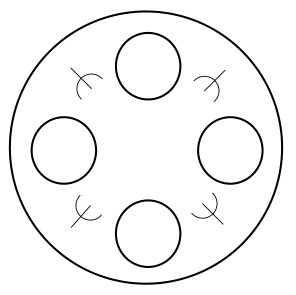
\includegraphics[scale=0.4]{img/preludiodidelus.png}
\end{figure}

Questo esempio ci permette di elencare tutte le condizioni necessarie affinchè si crei uno stallo:

\begin{enumerate}
    \item \textbf{Risorse limitate}: Una quantità infinita di risorse fornirebbe infatti la garanzia sull'assenza di stalli.
    \item \textbf{No Preemption}: Risorse assegnate non possono essere riassegnate.
    \item \textbf{Wait While Holding}: Nessuno lascia la propria risorsa, anche se è in fase di stallo.
    \item \textbf{Attesa Circolare}.
\end{enumerate}

\paragraph{Grafi di Holt} Possiamo rappresentare in questo modo la gestione di thread e risorse, individuando gli stalli con i cicli nel grafo:

\begin{figure}[htbp]
    \center
    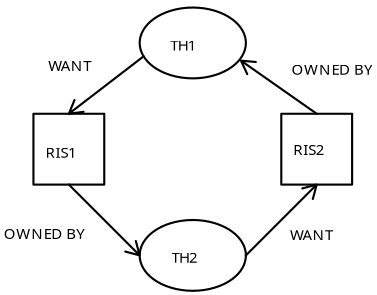
\includegraphics[scale=0.325]{img/grafoHolt.png}
\end{figure}

\subsubsection{Prevenzione e Cura degli Stalli}

Esistono delle politiche di prevenzione o di cura in caso occorressero degli stalli:

\begin{enumerate}
    \item \textbf{Detect and Fix - Politica di Cura Stallo}: Si analizza il Grafo di Holt e si interrompono i cicli effettuando kill dei thread scelti come vittime:
    \begin{figure}[htbp]
        \center
        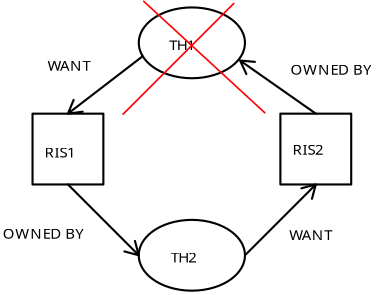
\includegraphics[scale=0.325]{img/kill_grafoHolt.png}
    \end{figure}
    Altrimenti posso eseguire politiche di \textbf{rollback} che grazie al salvataggio costante di uno stato di backup permette il ripristino nel caso in cui
    un operazione dovesse comportare una transizione a stato di stallo. Questa pratica comporta però dei costi in termini di mantenimento stato di backup.
    \newpage
    \item \textbf{Metodi di Prevenzione}: Esistono vari metodi che permettono la prevenzione di stalli, ad esempio:
    \begin{enumerate}
        \item Aumentare le risorse disponibili.
        \item Acquisire le risorse in un ordine imposto, ad esempio grazie ad una rigida enumerazione dei lock.
        \item Eliminare il Wait While Holding, un thread non potrà dunque holdare la risorsa durante uno stato non esecutivo.
        \item Acquisizione preventiva di tutte le risorse necessarie all'avvio dell'esecuzione del thread, altrimenti non si starta.
    \end{enumerate}
\end{enumerate}

\subsection{Algoritmo del Banchiere}

Descriviamo questo algoritmo che si pone l'obiettivo di riconoscere l'esistenza di almeno una schedulazione che attraversi solo stati safe, ossia stati deadlock free. Per
presentarlo abbiamo prima la necessità di definire le ipotesi su cui si basa:

\paragraph{Ipotesi dell'Algoritmo del Banchiere} Per la sua esecuzione si assumono validate queste condizioni:

\begin{enumerate}
    \item Si conosce il numero massimo di risorse richieste da un thread.
    \item Allocazione dinamica effettuata su richiesta (on-demand).
    \item Le richieste possono essere soddisfatte se esiste un ordinamento delle attività concorrenti dei thread/processi che sia deadlock free.
\end{enumerate}

\paragraph{Definizione di Stato Safe} Per qualunque sequenza di richieste di risorse tutte le attività concorrenti devono poter terminare. In maniera informale
possiamo dire che ogni stato deve avere a disposizione abbastanza risorse da far terminare almeno un thread in modo tale da causare il rilascio delle risorse che mantiene.
In questo modo, riconoscendo tanti stati safe consecutivi si identifica un path (traiettoria) che assicura l'esistenza di almeno una sequenza di stati safe che porta alla terminazione.
In questo modo viene effettuata un over-approssimazione sugli stati unsafe, saltando ogni stato unsafe anche se di transizione.

\paragraph{Complicazioni e Costi} La descrizione della traiettoria data sopra può aiutarci nel capire come per \textbf{ogni} stato safe esisterà
un tentativo di ricerca di traiettoria safe. In questo modo si riesce a capire la complessità causata da questo tipo di algoritmo che cerca di identificare ogni potenziale
traiettoria sicura.

\newpage

\subsubsection{Esempio d'Istanza e Rappresentazioni}

Mostriamo un esempio di transizioni tra stati:

\begin{enumerate}
    \item Tabella iniziale, seconda riga abbiamo la quantità di ciascun tipo di risorsa e le successive righe contengono la quantità di risorse divise per tipologia
    necessaria a ciascun thread per terminare:
    \vspace*{8px}
    \begin{center}
        \begin{tabular}{ |c|c|c|c| } 
         \hline
             & R1 & R2 & R3 \\ 
         \hline
             & 4 & 2 & 2 \\ 
         \hline
         th1 & 2 & 2 & 2 \\ 
         th2 & 3 & 1 & 1 \\ 
         th3 & 4 & 0 & 2 \\
         \hline
        \end{tabular}
    \end{center}
    \vspace*{8px}
    \item $th3$ richiede le risorse per terminare, e assumiamo che la parte di tabella inferiore non sia più
    riferita alle risorse necessarie ma quelle assegnate:
    \vspace*{8px}
    \begin{center}
        \begin{tabular}{ |c|c|c|c| } 
         \hline
             & R1 & R2 & R3 \\ 
         \hline
             & 0 & 2 & 0 \\ 
         \hline
         th1 & 0 & 0 & 0 \\ 
         th2 & 0 & 0 & 0 \\ 
         th3 & 4 & 0 & 2 \\
         \hline
        \end{tabular}
    \end{center}
    \vspace*{8px}
    Quindi $th2$ riesce a terminare.
    \item Lo stato successivo sarà dunque:
    \vspace*{8px}
    \begin{center}
        \begin{tabular}{ |c|c|c|c| } 
         \hline
             & R1 & R2 & R3 \\ 
         \hline
             & 4 & 2 & 2 \\ 
         \hline
         th1 & 0 & 0 & 0 \\ 
         th2 & 0 & 0 & 0 \\ 
         \hline
        \end{tabular}
    \end{center}
    \vspace*{8px}
    E continuando in questo modo sarà possibile identificare o meno una traiettoria che porta alla conclusione di tutti i threads.
\end{enumerate}

\newpage

\subsubsection{Pseudocodice dell'Algoritmo del Banchiere}

Mostriamo una possibile implementazione dell'Algoritmo del Banchiere:

\vspace*{10px}

\begin{lstlisting}[language = C]
    while(esiste un thread non marcato){
        if(esiste un altro thrd-i tale che esigenza_i <= d){
            marco thread-i
            rimetto nella disponibilta le risorse assegnate al thrd-i
        } else {
            stato non safe //blocco, NON si assegna la risorsa al thrd-i
        }
        stato safe
        procedi
    }
\end{lstlisting}

\subsection{Scheduling}

Fino ad ora abbiamo solo menzionato come lo scheduling venisse gestito da una serie di transizione di stati in base agli eventi accaduti. In questo capitolo
elencheremo delle definizioni e successivamente delle vere e proprie politiche di scheduling.

\paragraph{Definizioni} Elenchiamo delle definizioni utilizzate nella gestione dello scheduling:

\begin{enumerate}
    \item \textbf{Task/Job}: Attività da completare.
    \item \textbf{Latency/Response Time}: Velocità del tempo di risposta, importante in schemi che danno priorità all'interattività, nello specifico:
    \begin{enumerate}
        \item \textbf{Latency}: Tempo che intercorre dall'inizio alla fine di un task.
        \item \textbf{Response Time}: Tempo che intercorre dall'istante iniziale a quando ottengo l'esito del task.
    \end{enumerate}
    \item \textbf{Throughput}: Esecuzione di più task in contemporanea in un quanto di tempo.
    \item \textbf{Predictability}: Vincolo di rispettare tempi in casi specifici, come contesti realtime.
    \item \textbf{Overhead}: Quanto tempo impiego in più a causa della gestione della schedulazione, ossia azioni come:
    \begin{enumerate}
        \item Cambiare stato.
        \item Aggiungere in coda.
        \item Effettuare commutazioni di contesto.
    \end{enumerate}
    \item \textbf{Fairness}: Quanto risulta equa la performance ottenuta per ciascun user.
    \item \textbf{Workload}: Set di task per sistema da dover completare. Spesso questo viene utilizzato in contesti che non danno importanza ad un alta interattività ma alle performance (contesti di number crunching).
\newpage
    \item \textbf{Pre-Emptive Scheduler}: Permesso il prerilascio di risorse già assegnate ad un task, se una priorità di task già in esecuzione dovesse risultare più bassa di un task in entrata allora
    scheduler ha il permesso di riassegnare la risorsa contesa.
    \item \textbf{Scheduling Algorithms}: Algoritmi che ricevono in input i dettagli del contesto e producono in output il modo in cui gestire la schedulazione.
\end{enumerate}

\subsubsection{Politiche di Schedulazione}

Esistono vari modi per gestire la schedulazione di task:

\begin{enumerate}
    \item \textbf{FIFO}: Workload composto di task che vengono schedulati in base all'ordine in cui arrivano, seguono quindi un ordine settato da una coda, per questo 
    
    è detta \textbf{politica FIFO}.
    \vspace*{-10px}
    \paragraph{Caratteristiche} Questa politica non valuta il tempo di completamento dei task. Di conseguenza i task più brevi se entrassero dopo task più lunghi dovrebbero aspettare tutta l'esecuzione di questi, dando poca importanza quindi all'interattività.
    \item \textbf{Shortest Job First (SJF)}: Viene data priorità ai task più brevi.
    \begin{enumerate}
        \item \textbf{Non Pre-Emptive}: Lista ordinata sui tempi di completamento dei \textbf{READY}. Non prendiamo in considerazione dunque i thread in stato di \textbf{EXEC}.
        \item \textbf{Pre-Emptive}: Oltre alla lista ordinata sui \textbf{READY}, in questa versione di (SJF) se un nuovo task ha un tempo di completamento inferiore al corrente task in stato di \textbf{EXEC} allora il task in esecuzione viene sostituito dal task in entrata. 
    \end{enumerate}
    \vspace*{-10px}
    \paragraph{Caratteristiche} Analizziamo pro e contro di questa politica di scheduling:
    \begin{enumerate}
        \item \textbf{Pro}: Buona response time media, ottimale nell'essere responsive.
        \item \textbf{Contro}: Si presentano una serie di contro:
        \begin{enumerate}
            \item Overhead causato dalle frequenti operazioni di schedulazione come le commutazioni.
            \item Potenziali lunghe posticipazioni in condizioni specifiche come un task lungo seguito da task lunghi quasi quanto il primo.
            \item A priori dovremmo conoscere il tempo d'esecuzione di un thread/processo.
            \item Varianza alta nel tempo di risposta.
        \end{enumerate}
    \vspace*{5px}
    \item \textbf{Round Robin}: Politica basata sulla \textbf{divisione} in \textbf{quanti} di \textbf{tempo} di task e l'esecuzione di questi risulterà indipendente dalla durata dei task a cui appartengono.
    \vspace*{-10px}
    \paragraph{Scelta Durata Quanto di Tempo} La scelta della durata di un quanto di tempo sarà influenzata da vari elementi:
    \begin{enumerate}
        \item Un quanto di tempo corto causerebbe un comportamento simile ad una (SJF) mentre uno lungo risulterebbe simile ad una FIFO.
        \item Il quanto di tempo sarà gestito anche in base al tipo di computazione, alte prestazioni richiederebbero un ampio quanto, mentre alta interattività richiederebbe un breve quanto.
    \end{enumerate}
    \end{enumerate}
\end{enumerate}

\newpage

\subsubsection{Multi Level Feedback Queue}

Per rendere la \textbf{schedulazione} il più \textbf{fair} possibile è necessario che ogni tipologia
di job nel workload (CPU Bounded o I/O Bounded) abbia la stessa possibilità di essere schedulato.
Una normale applicazione di una politica di Round Robin potrebbe infatti causare una schedulazione non fair nei confronti
dei processi I/O Bounded.

\paragraph{Obiettivi} Questo approccio si basa su un insieme di code caratterizzate da priorità diverse. Questo meccanismo vuole garantire:

\begin{enumerate}
    \item Migliorare i tempi di risposta.
    \item Bassa overhead.
    \item Diminuzione di casi di starvation.
    \item Possibilità di caratterizzare un task con un livello di priorità alta/bassa.
    \item Essere il più fair possibile su task caratterizzati dallo stesso livello di priorità.
\end{enumerate}

\paragraph{Caratteristiche} Questo meccanismo si basa su questi elementi fondamentali:

\begin{enumerate}
    \item Struttura di code, ciascuna con priorità diversa.
    \item Priorità più alte hanno quanti di tempo più brevi.
    \item Schedulatore estrae task da eseguire sempre dalla coda con almeno un elemento e di priorità più alta disponibile.
    \item Meccanismo di feedback che dia la possibilità di spostare un task da una coda ad un altra in base a specifici indici.
    \item Uno schema di \textbf{posizionamento} di \textbf{task} nelle \textbf{code}:
    \begin{enumerate}
        \item Task in entrata vengono \textbf{posizionati} sempre a \textbf{priorità} più \textbf{alta}.
        \item Task che si \textbf{sospendono} (come per yield o I/O) \textbf{restano} al loro \textbf{livello} oppure \textbf{crescono}.
        \item Task che \textbf{esauriscono} il loro quanto di tempo passano al \textbf{livello sottostante}.
    \end{enumerate}
\end{enumerate}

\paragraph{Esempio di Gestione a Code di Priorità - Windows}

Windows posiziona i propri task in $32$ code di schedulazione suddivise in \textbf{system} e \textbf{user}:

\begin{enumerate}
    \item Viene data la priorità ai task lato system.
    \item Ai task in entrata di tipo user viene dato un livello pari ad $8$:
    \begin{enumerate}
        \item Se questo appartiene ad operazione di I/O allora viene incrementata la priorità in base al tipo di I/O.
        \item Se riattivata da una wait (operazione di sync) allora:
        \[ \text{da Background} \: \mapsto +1 \:\:\:\:\: \text{da Foreground} \: \mapsto +2 \:\:\:\:\: \text{se usa tutto il quanto} \: \mapsto -1 \]
    \end{enumerate}
\end{enumerate}

\newpage

\paragraph{Inversione di Priorità} Potrebbe risultare utile menzionare questa condizione per cui un task appartenente ad una coda di priorità alta si metta in attesa di un task contenuto in una coda
a priorità minore.

\paragraph{Riepilogo Caratteristiche Politiche di Schedulazione} Piccolo riepilogo delle caratteristiche delle politiche descritte sopra:

\begin{enumerate}
    \item \textbf{FIFO}: Gestione semplice a coda:
    \begin{enumerate}
        \item Task di lunghezza variabile porta task brevi ad attendere task lunghi.
        \item Task di lunghezza costante è un ottima politica di scheduling.
    \end{enumerate}
    \item \textbf{Shortest Job First}: Gestione a coda ordinata per tempo di esecuzione:
    \begin{enumerate}
        \item Ottima per la media di tempo di risposta.
        \item Pessima per varianza di tempo di risposta.
        \item Risulta necessario conoscere il tempo d'esecuzione di un task.
    \end{enumerate}
    \item \textbf{Round Robin}: Gestione "migliore" o più nello specifico gestione che ci permette di definire in maniera personalizzata i quanti di tempo. Abbiamo però visto
    come risulti necessario utilizzare sistemi di code di priorità per rendere la politica fair.
\end{enumerate}

\subsubsection{Schedulazione Multi-Processor}

Descriviamo le politiche di schedulazione su architetture Multi-Processor:

\paragraph{Scheduling Oblivious} I thread che compongono i processi in questa politica vengono assegnati a core indipendentemente dal processo a cui appartengono. In questo modo lo scheduler non è a conoscenza della disponibilità di core diversi, semplicemente \textbf{schedula thread} su \textbf{core} in \textbf{maniera arbitraria}.
Dunque thread dello stesso processo potrebbero essere schedulati su core diversi e questo potrebbe causare una gestione pesante dei dati tra le varie cache dei core, ma resta lo schema più semplice.
Questo tipo di scheduling presenta diversi punti di debolezza:

\begin{enumerate}
    \item Produce delay in caso di utilizzi di BSP e Producer/Consumer.
    \item Produce delay in casi di path critici.
    \item Produce I/O delay su alcuni threads.
\end{enumerate}

\paragraph{Affinity Scheduling} Ogni core ha la propria MCQ, e di conseguenza si riposizionano i threads nella lista pronti da dove sono stati estratti più recentemente. I processori in idle possono fare \textbf{stealing} di task di altri core per bilanciare il workload tra i core. L'obiettivo è quello di bilanciare il workload mantenendo più affinità di cache possibile.

\newpage

\paragraph{Pattern di Programmazione Multithread} Nella programmazione multithread 

riconosciamo dei pattern di utilizzo:

\begin{enumerate}
    \item \textbf{(BSP) - Bulk Synchronous Parallel}: Normalmente i thread comunicano durante il loro corso d'esecuzione. In questo pattern invece si crea una barriera che imposta un \textbf{momento} di \textbf{comunicazione sincronizzato}.
    \begin{figure}[htbp]
        \center
        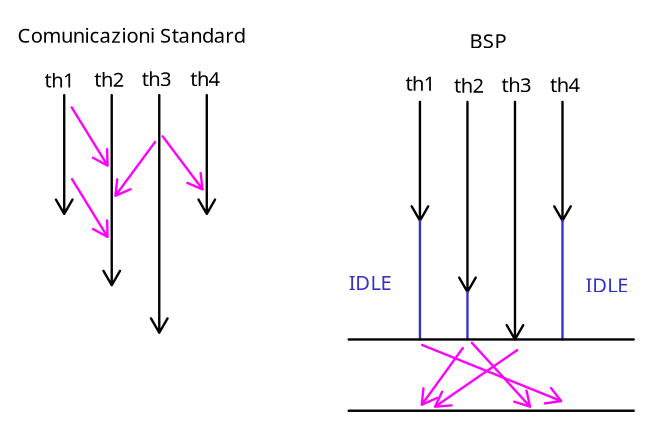
\includegraphics[scale=0.35]{img/BSP.png}
    \end{figure}
    Lo schema BSP si compone dunque di due fasi:
    In generale quindi questo pattern crea la necessità di dover gestire i tempi di idle, magari deschedulando questi thread.
    
    \begin{enumerate}
        \item \textbf{Fase Superstep}: I thread sono in esecuzione fino al loro completamento, tutti i thread che non sono quelli con il maggior tempo di completamento passano ad uno stato di idle in attesa del completamento del più lungo.
        \item \textbf{Fase Comunicazione}: Tutti i thread comunicano tra loro in maniera sincrona.
    \end{enumerate}
    \item \textbf{Pipeline - Produttore/Consumatore}: La pipeline si basa su entità consecutive, ciascuna basa il proprio input sull'output di quello precedente, come nel processore pipeline appunto che
    si basava su fasi come $FETCH, DECODE, EXEC$. Dunque il pattern si basa sui producer che pushano dati in un buffer ed i producer estraggono dati dal buffer.
\end{enumerate}

\paragraph{Gang/Space Scheduling} Descriviamo questi tipi due tipi di scheduling:

\begin{enumerate}
    \item \textbf{Gang Scheduling}: Si tenta di schedulare tutti i thread appartenenti ad un processo, altrimenti non lo si manda in esecuzione.
    \item \textbf{Space Scheduling}: Si schedulano diversi task di processi a diversi core.
\end{enumerate}

\paragraph{Problema del Cammino Minimo} Ogni nodo rappresenta un thread e un arco una dipendenza. Il cammino critico corrisponde al \textbf{cammino più lungo} in termini di tempo dalla radice alla foglia.

\newpage

\section{Traduzione Indirizzi}

I punti fondamentali di questo capitolo saranno: concetto di \textbf{Traduzione di Indirizzi}, \textbf{Traduzione Flessibile di Indirizzi} (Virtual Base and Bound, Segmentazione, Paginzazione e Traduzione Multilivello) e \textbf{Traduzione di Indirizzi Efficiente}.

\paragraph{Proprietà del Mapping} La gestione della memoria basata su mapping virtuale-fisico offre queste proprietà:

\begin{enumerate}
    \item Protezione grazie all'isolamento di specifiche zone della zona di memoria.
    \item Sharing di memoria.
    \item Flessibilità.
    \item Indirizzi sparsi su spazio fisico e loro gestione.
    \item Portabilità.
    \item Efficienza.
\end{enumerate}

Oltre a questo la virtualizzazione della memoria permette:

\begin{enumerate}
    \item Isolamento della memoria.
    \item Inter Process Comunicate.
    \item Shared Memory tra Processi.
\end{enumerate}

L'unità che si occuperà della traduzione degli indirizzi è l'MMU. Questa unità dato un indirizzo logico lo tradurrà in uno fisico in base ad uno schema seguito. Fondamentale sarà anche il posizionamento dell'MMU, infatti il posizionamento (prima o dopo il primo livello di cache) influisce fortemente sulla tipologia di approccio seguito.

\subsection{Base and Bound, Segmentazione, Paginazione}

\paragraph{Virtual Base and Bound} Si definisce una base ed un offset nell'MMU che ricevuto un indirizzo virtuale controllerà se questo è contenuto nell'intervallo definito, formalmente: 

\vspace*{-10px}

\[ indirizzo + base < base + bound \]

\begin{figure}[htbp]
    \center
    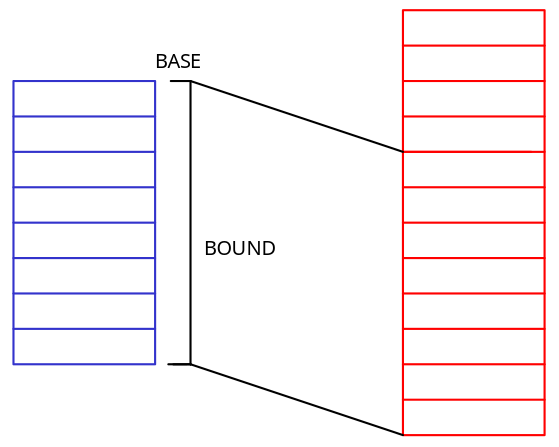
\includegraphics[scale=0.3]{img/base_and_bound.png}
\end{figure}

\newpage

\paragraph{Partizioni Variabili e Base and Bound} Questo schema forma partizioni variabili nel tempo, e questo causa un fenomeno di \textbf{frammentazione esterna}, 
ossia spazio non ancora allocato "più piccolo" posizionato esternamente alle zone di memoria fisiche allocate per i processi. Questo spreco di spazio in memoria fisica è risolvibile grazie ad una \textbf{traslazione} di tutti i \textbf{blocchi allocati} per i processi. Questo fenomeno è detto \textbf{deframmentazione}.

\paragraph{Segmentazione}

Si suddividono gli \textbf{indirizzi logici} in \textbf{segmenti}, mantenendo per ciascun segmento una coppia di valori $(base, bound)$. Quindi avremo ad esempio un segmento codice, un segmento dati ed uno dati dinamici che andranno gestiti \textbf{ciascuno} con una \textbf{specifica coppia} di $(base, bound)$.

\begin{figure}[htbp]
    \center
    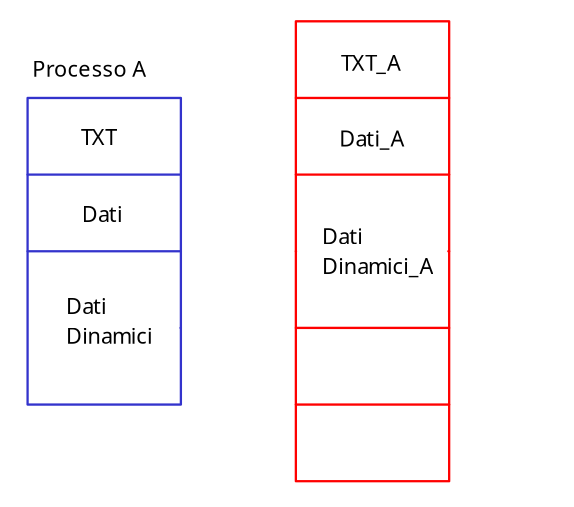
\includegraphics[scale=0.35]{img/segmentazione.png}
\end{figure}

Questo approccio ha dei pro come potenziale condivisione di segmenti tra processi, protezione, crescita fino alla dimensione necessaria dello stack/heap, però causa una gestione più complessa dato che va cercato durante ogni allocazione di segmento una dimensione specifica di memoria libera ed oltre a questo causa \textbf{frammentazione esterna}.

\paragraph{Paginazione} In questo approccio si suddivide tutto lo spazio d'indirizzamento di un processo in unità di pari dimensioni.

\begin{figure}[htbp]
    \center
    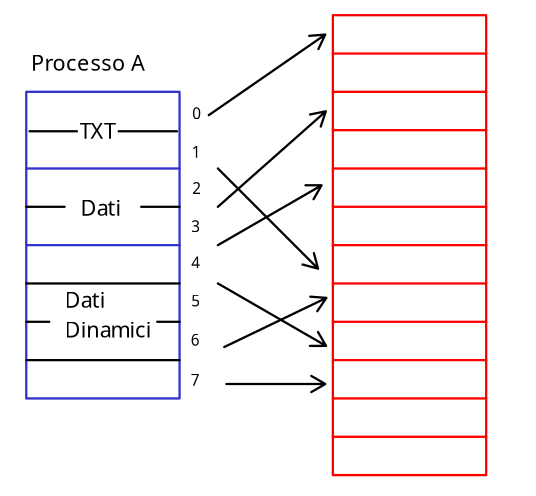
\includegraphics[scale=0.3]{img/paginazione.png}
\end{figure}

Questo schema non presenta problemi di frammentazione esterna ma di frammentazione interna (ossia spazio perso all'interno delle pagine), la gestione della MMU risulta però semplice, dato che corrisponderà solo ad una somma di indirizzi logici come multipli di $2$.

\newpage

\paragraph{Translation Lookaside Buffer (TLB) in una MMU in Paginazione} Nel caso della gestione a paginazione della traduzione di indirizzi è necessaria una rete che dato in input un indirizzo (composto da numero di pagina logica ed offset) sia in grado di restituire in maniera completamente associativa il corrispondente indirizzo fisico. Questa rete è chiamata \textbf{TLB}
e nello schema di paginazione è molto simile ad una cache completamente associativa.

\subsection{Segmentazione Paginata}

Questo schema di traduzione cerca di sfruttare i pro di entrambe le tipologie di traduzione viste prima, cercando un \textbf{compromesso} tra le due. Lo \textbf{spazio d'indirizzamento} di un \textbf{processo} sarà diviso in \textbf{segmenti} che saranno a loro volta \textbf{divisi} in \textbf{pagine}.

\begin{figure}[htbp]
    \center
    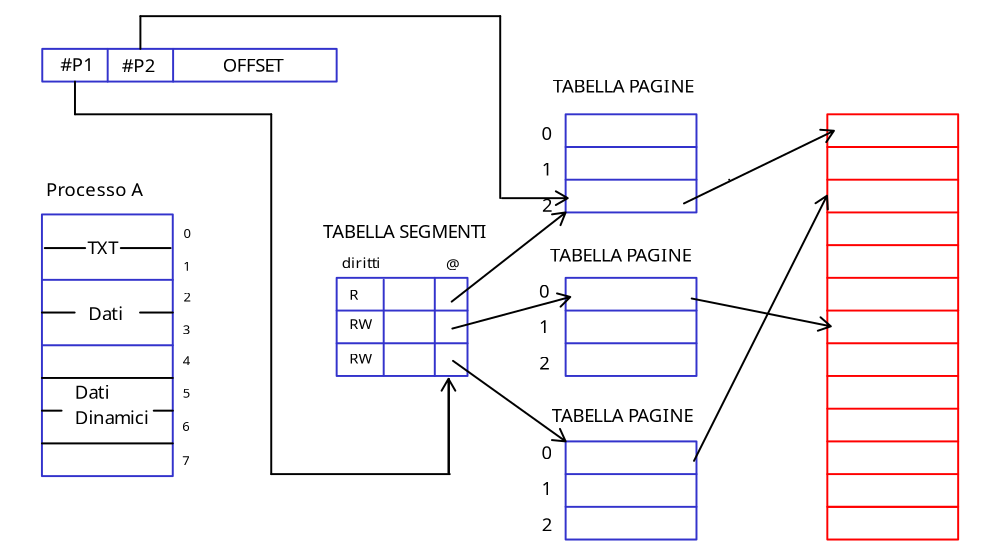
\includegraphics[scale=0.3]{img/segmentazione_paginata.png}
\end{figure}

Vediamo in questo modo come si compone un vero e proprio albero di tabelle di \\ traduzione.
Questo permette un allocazione della memoria più efficiente. Questo caso rappresentato è tra i più semplici, infatti potrebbero esserci $k$ livelli di tabelle di pagine.

\paragraph{Interpretazione degli Indirizzi} Mostriamo in che modo vengono interpretati gli indirizzi e quali sono le caratteristiche di ciascuna tipologia:

\[ IND\_LOG \:\: = \:\: < PAG\_LOG, OFFSET> \]

\vspace*{-15px}

\[ IND\_FIS \:\: = \:\: TAB\_PAG[PAG\_LOG] * AMPIEZZA\_PAG + OFFSET \]

Quindi un indirizzo logico sarà composto da pagina logica e offset, la pagina logica viene utilizzata per indicizzare nella tabella delle pagine e di conseguenza
l'indirizzo fisico sarà la dereferenziazione in tabella delle pagine dell'indice dato dal numero di pagina logica più l'offset copiato dall'indirizzo logico. 
\vspace*{5px}


La scelta di quanti bit dedicare al numero di pagina e all'offset nel indirizzo logico porta a due vie:

\begin{enumerate}
    \item \textbf{Pochi bit per pagina logica, tanti per offset}: Causa frammentazione interna.
    \item \textbf{Pochi bit per offset, tanti per pagina logica}: Causa tabelle di pagine molto grandi.
\end{enumerate}

\newpage

\subsubsection{Gestione a più Tabelle di Pagine e Commutazione di Contesto} Analizziamo queste due specifiche condizioni che possono presentarsi nella gestione della traduzione degli indirizzi:

\paragraph{Gestione Multi Tabella di Pagine} Se nell'interpretazione di un indirizzo logico considerassimo non un singolo blocco dedicato all'indice di tabella di pagine bensì due allora avremmo una gestione multipagina che utilizzerà
questi due campi come indici nelle tabelle. Come nello schema classico il resto bit saranno dedicati all'offset utilizzato per spostarsi nella pagina fisica finale.

\paragraph{Commutazione di Contesto} Ipotizziamo una condizione per cui si verifica una commutazione di contesto. La CPU dovrà quindi passare dall'esecuzione del Processo A a quella del Processo B. In qualche modo quindi sarà necessario cambiare le informazioni contenute nella TLB, esistono due diversi approcci con caratteristiche diverse:

\begin{enumerate}
    \item Si effettua il flush della TLB, rimuovendo quindi tutte le informazioni di traduzione di indirizzi riguardanti il Processo A. Questo è semplice da implementare ma non cerca di preservare informazioni di traduzione che potrebbero risultare utili dopo.
    \item Nella TLB si mantiene una coppia di informazioni, ossia numero di pagina logica e pid a cui appartiene. In questo modo si fornisce una possibilità riguardo il mantenimento di pagine "vecchie" durante una commutazione, questo comporta allo stesso tempo un implementazione un po' più complessa nella logica della TLB.
\end{enumerate}

\subsubsection{Cache Virtuale/Fisica}

Non abbiamo definito ancora formalmente dove viene posizionata l'MMU, se dopo o prima il primo livello di cache. Questa scelta risulta infatti importante
nell'interpretazione degli indirizzi. Esistono questi due tipi di gestione:

\begin{enumerate}
    \item \textbf{Cache Fisica}: Dato un \textbf{indirizzo logico} generato dalla CPU, questo verrà \textbf{prima tradotto} dall'MMU (con relativa TLB) e \textbf{successivamente} dato in \textbf{input} alla cache \textbf{sotto forma} di \textbf{indirizzo fisico}.
    
    Questa implementazione causa un costo di traduzione.
    \item \textbf{Cache Virtuale}: Dato un \textbf{indirizzo logico} generato dalla CPU, questo lo si usa \textbf{direttamente} in cache, ma va interpretato nel modo corretto, assumendo che ogni entry abbia specifici campi come $\{tag, pid, p, m, b parole\}$ e dunque la chiave utilizzata nel confrontatore della cache sarà definita da entrambi i campi $\{tag, pid\}$. Questa gestione causa un costo inferiore ma delle complicazioni causate dalla gestione del pid, dato che non esiste nessuna istruzione
    primitiva che permetta la sua gestione diretta.
\end{enumerate}

Di conseguenza il \textbf{tipo} di \textbf{cache} è definito dal \textbf{tipo} di indirizzo \textbf{che acquisisce} in \textbf{input}.

\newpage
\subsubsection{Core Map e Gestione Tabelle di Pagine}

Seguendo lo schema mostrato fino ad ora, risulterebbe necessario mantenere nella tabella delle pagine un numero di indirizzi a pagine pari a quante sono la somma di tutte le pagine logiche di tutti i processi. Vorremmo
però mantenere solo le reali pagine, ossia gli indirizzi delle pagine fisiche. 



Immaginiamo dunque una hashtable di pagine con i seguenti campi per riga:

\begin{enumerate}
    \item Numero di pagina.
    \item Pid del processo a cui appartiene.
    \item Puntatore al next (gestione della collisione per questa hashtable).
\end{enumerate}

\begin{figure}[htbp]
    \center
    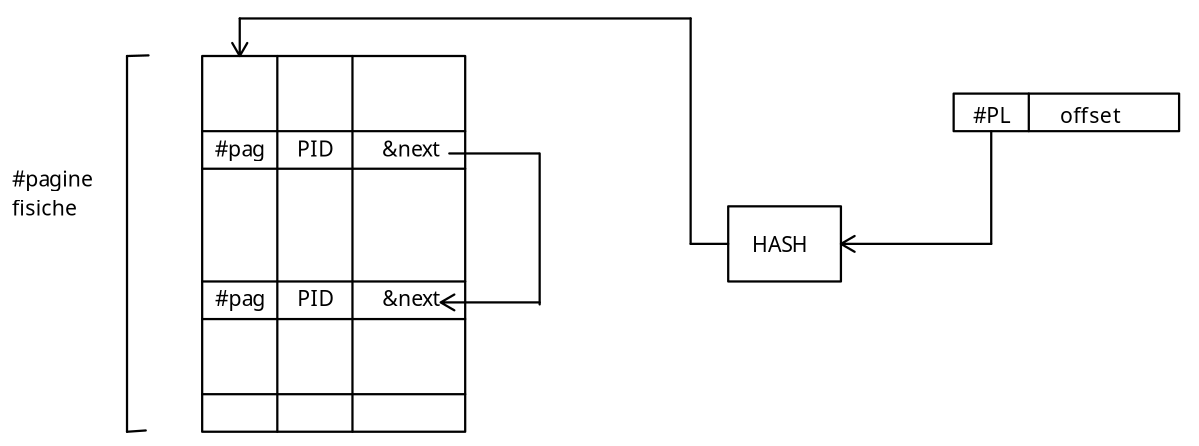
\includegraphics[scale=0.25]{img/coreMap.png}
\end{figure}


In questo modo, dato in input un indirizzo, questo viene dato alla funzione di hash e il suo output verrà utilizzato per indicizzare l'accesso alla tabella.
Grazie all'utilizzo del PID contenuto nella riga riusciamo a stabilire se quella pagina appartiene o meno al corrente processo, infatti se il PID non corrispondesse a quello atteso si dereferenzierebbe il campo next fino all'ultima riga caratterizzata da quel valore di hash.

\subsection{Elementi in Dettaglio di Gestione di Memoria Virtuale}

Dopo aver definito la gestione a paginazione della memoria virtuale, analizziamo in dettaglio alcuni elementi e fenomeni che la caratterizzano.

\paragraph{Descrittore di Pagina} Un descrittore di pagina permette di mantenere una serie di informazioni riguardanti una pagina:

\begin{enumerate}
    \item Numero di pagina fisica in memoria o info riguardanti la posizione su disco.
    \item Permessi d'accesso (Bit Read e Write).
    \item Bit Modifica (M) utile nella gestione del page fault.
    \item Bit Utilizzo (U) utile nella gestione del page fault.
    \item Bit Presenza (P), ossia $1$ se la pagina è in memoria e $0$ se è sul disco. 
\end{enumerate}

Questo oggetto permetterà alcune operazioni (come la paginazione On-Demand, ossia la richiesta in memoria di una pagina su disco) in maniera regolare, seguendo i parametri che descrivono la pagina stessa nel suo descrittore.

\newpage

\subsubsection{Page Fault e Page Replacement}

Seguendo lo schema impostato fino ad ora, la memoria principale fa da vera e propria cache al disco, di conseguenza possono occorrere anche dei fault.

\paragraph{Page Fault} Descriviamo in fasi il page fault:

\[ Proc_{A} \text{ riferisce a } < pag\_logica, offset > \:\: \rightarrow \:\: \nexists \: pag\_fisica \text{ in memoria} \]

\begin{enumerate}
    \item La CPU genera un indirizzo logico.
    \item Si da in input l'indirizzo logico alla MMU ed al relativo TLB.
    \item Il TLB trova il bit di presenza relativo all'indirizzo passato pari a $0$ (passando prima per la tabella delle pagine e poi per la memoria effettiva), di conseguenza genera un fault.
\end{enumerate}

Questo fault però implica che se la pagina non è stata trovata allora la si vuole caricare dal disco alla memoria, di conseguenza vengono effettuati questi ulteriori passaggi per il \textbf{caricamento} di \textbf{pagina} \textbf{dal disco alla memoria}:

\begin{enumerate}
    \item Si trova un indirizzo in core map che sia libero (free).
    \item Si prende dal disco la pagina $PL$ che ha causato il fault in memoria e la si carica all'indirizzo indicato come (free) nella core map.
    \item Si posiziona in memoria fisica la pagina presa dal disco.
    \item Va aggiornata la tabella delle pagine.
    \item Si modifica la core map, indicando che la posizione non è più (free).
\end{enumerate}

Tutta questa procedura sarà effettuata come un vero e proprio \textbf{handling} di \textbf{eccezione} causato dal \textbf{fault}. Di conseguenza dopo la sua esecuzione sarà necessario poter tornare all'istruzione successiva a quella che ha causato il fault stesso (LDR/STR/FETCH).

\vspace*{10px}

\paragraph{Page Replacement}

Nel caso in cui non sia presente abbastanza spazio tra le pagine allocate in memoria, si effettua un \textbf{operazione} di \textbf{rimpiazzamento} di pagina
basata sulla \textbf{rimozione} di una \textbf{specifica pagina} indicizzata, ad esempio, da $y$ nella Core Map.

\vspace*{10px}

Elenchiamo a pagina successiva le fasi di questa procedura.

\newpage

\begin{enumerate}
    \item Si identifica l'indice $y$ nella Core Map della $pagina_{z}$ vittima che \\ appartiene ad un $processo_{A}$.
    \item Si prende rispettiva pagina fisica in memoria, appunto $pagina_{z}$.
    \item Questa pagina avrà una relativa posizione sul disco, allora:
    \begin{enumerate}
        \item Se il bit $M$ nel descrittore di pagina è $1$ allora porto la pagina vittima sul disco, dato che sono state apportate modifiche rispetto alla sua versione originale.
        \item Se il bit $M$ nel descrittore di pagina è $0$ allora rimuovo semplicemente la pagina.
    \end{enumerate}
    \item Nella tabella delle pagine del $processo_{A}$ si inserisce ad indice $z$ il bit di presenza $P=0$, dato che è stata rimossa.
    \item Nella Core Map viene settata a $free$ l'indice $y$.
\end{enumerate}

Questo fenomeno di Page Replacement può essere causato dal fenomeno di Page Fault descritto prima nel momento in cui, a tempo di caricamento di pagina, non fosse disponibile spazio in memoria.

\paragraph{Implementazione dei Bit M ed U} Esistono due modi per implementare i bit $M$ ed $U$ nel descrittore, l'implementazione può essere infatti \textbf{Hardware} o \textbf{Software}:

\begin{enumerate}
    \item \textbf{Implementazione Hardware}: I bit $M$ ed $U$ vengono mantenuti nel descrittore di pagina, dunque saranno attributi di ciascuna entry della TLB. Questa implementazione risulta meno costosa rispetto a quella proposta dopo.
    \item \textbf{Implementazione Software}: Non è presente il meccanismo degli attributi delle entry della TLB, di conseguenza risulterà necessario emulare il comportamento dei due bit.
    Elenchiamo un paio di possibili casistiche ed emulazione dei due bit:
    \begin{enumerate}
        \item Se avessi una pagina con $R=1$ e $W=0$ allora tentare una $STR$ causerebbe un eccezione a causa dei meccanismi di protezione. Di conseguenza bisogna emulare $M$ settando ad esempio tutti i $W=0$ per fare in modo che l'handling della prima eccezione mi setta $W=1$ e $M=1$.
        \item Allo stesso modo potrei gestire anche il bit $U$, settando tutte le pagine di default come non valide ($P=0$), dunque tutte le operazioni come $LDR, \: STR, \: FETCH$ causeranno delle eccezioni il cui handler si occuperà del setting delle flag $P=1, \: U=1$.
    \end{enumerate}
    Questo può causare un costo leggermente più alto nella gestione di questi due bit dato che sarà necessario utilizzare il meccanismo di handling delle eccezioni qualora siano necessari i bit $M$ ed $U$.
\end{enumerate}

\newpage

\subsubsection{Politiche di Selezione dell'Indice di Pagina Vittima}

Durante il Page Replacement abbiamo menzionato un indice $y$ arbitrario, che indicava la pagina identificata come vittima nella Core Map. Stabiliamo in questo capitolo le politiche di selezione di questo indice:

\begin{enumerate}
    \item \textbf{Politica Random}: Selezione casuale dell'indice, questo può risultare semplice da implementare ma poco efficiente in quanto a prestazioni.
    \item \textbf{Politica FIFO}: Si segue un ordine FIFO rispetto al accesso di pagina logica:
    \begin{center}
        \begin{tabular}{ |c|c|c|c|c|c|c|c|c|c|c| } 
         \hline
           & A & B & C & D & E & A & B & C & D & E \\ 
         \hline
         1 & A &  &  &  & E &  &  &  & D &  \\ 
         \hline
         2 &  & B &  &  &  & A &  &  &  &  E \\ 
         \hline
         3 &  &  & C &  &  &  & B &  &  &  \\ 
         \hline
         4 &  &  &  & D &  &  &  & C &  &  \\ 
         \hline
        \end{tabular}
        \end{center}
    Questa politica in questo caso non è molto efficiente data la bassa disponibilità di pagine fisiche disponibili. Nella tabella infatti la prima colonna rappresenta le pagine fisiche disponibili e la prima riga l'accesso alle pagine logiche.
    \item \textbf{Politica Min}: In caso di mancanza di pagine fisiche sostituisco quella che riferirò nel futuro più tardi:
    \begin{center}
        \begin{tabular}{ |c|c|c|c|c|c|c|c|c|c|c| } 
         \hline
           & A & B & C & D & E & A & B & C & D & E \\ 
         \hline
         1 & A &  &  &  &  &  &  &  &  &  \\ 
         \hline
         2 &  & B &  &  &  &  &  &  &  &   \\ 
         \hline
         3 &  &  & C &  &  &  &  &  & D &  \\ 
         \hline
         4 &  &  &  & D & E &  &  &  &  &  \\ 
         \hline
        \end{tabular}
        \end{center}
    Questo algoritmo è ottimo ma allo stesso tempo ideale dato che si suppone di conoscere a priori quando verrà richiesta una pagina logica.
    \item \textbf{Politica LRU}: Come definito dalla sigla, questa politica sceglie il criterio Least Recently Used, sul lungo termine può assomigliare molto ad una FIFO.
    \item \textbf{Politica NRU}: Come già visto nel capitolo delle cache, la politica Not Recently Used sfrutta dei bit d'uso settati a $0$ di default e messi ad $1$ in caso di accesso alla pagina, effettando dei periodici refresh di tutte le pagine a $0$. Questo ci permette di tenere traccia delle pagine verso cui si effettuano più accessi, in modo tale da scegliere vittime che non causino futuri caricamenti di pagine appena rimosse.
    \item \textbf{Algoritmi di Approssimazione di LRU}: Elenchiamo una serie di algoritmi che puntano ad approssimare l'LRU descritto prima:
    \begin{enumerate}
        \item \textbf{Algoritmo Second Chance}: Ad ogni pagina è associato un contatore ed ogni ricerca di pagina vittima passa in "senso circolare" su tutte le $pagine_{i}$ controllando il valore del contatore:
        \begin{enumerate}
            \item Se $contatore_{i} > 0$ allora $contatore_{i} = contatore_{i} - 1 $.
            \item Se $contatore_{i} = 0$ allora $pagina_{i}$ è scelta come vittima.
        \end{enumerate}
\newpage
        \item \textbf{Algoritmo del Working Set}: Viene definito un tempo $T$ che definisce \\ l'intervallo in cui se una specifica pagina non viene riferita allora è fuori dal Working Set. Ogni pagina si porta dietro tre specifici attributi:
        \begin{enumerate}
            \item \textbf{Bit di Riferimento}: definisce se la pagina è stata riferita o meno.
            \item \textbf{TLR}: Tempo approssimato dall'ultimo riferimento.
            \item \textbf{AGE}: $\text{Tempo Corrente} - \text{TLR}$.
        \end{enumerate}
        Questo algoritmo segue questi passi:
        \begin{enumerate}
            \item Per ogni pagina:
            \begin{enumerate}
                \item Se $R=0$ allora $AGE = \text{Tempo Corrente} - \text{TLR} $
                \item Se $R=1$ allora $AGE = \text{Tempo Corrente}$ e $R = 0$.
            \end{enumerate}
            \item Se una pagina:
            \begin{enumerate}
                \item Ha $AGE < T$ allora è nel Working Set.
                \item Ha $AGE \geq T$ allora è candidata per la rimozione.
            \end{enumerate}
        \end{enumerate}
        Questi due \textbf{passi} vengono \textbf{eseguiti} in \textbf{maniera sequenziale} per ciascuna pagina in senso circolare per identificare delle pagine vittime. Questo algoritmo può essere utilizzato anche per mantenere un pool di pagine libere correlate alla dimensione attesa del Working Set, in modo tale da garantire sempre spazio per la pagina da caricare. Questa \textbf{politica} del \textbf{pool} va però gestita perchè può portare anche a svantaggi di overhead se di dimensioni troppo estese.
    \end{enumerate}
\end{enumerate}

\subsubsection{File Memory Mapped}

Astrazione caratteristica del mondo UNIX, che ci permette di rendere un file la virtualizzazione di segmenti di memoria condivisa. Nello specifico immaginiamo questi specifici passi:

\begin{enumerate}
    \item Viene aperto un file, tramite una \textbf{open}, da \textbf{due diversi processi}.
    \item \textbf{Non vogliamo} un \textbf{apertura} di \textbf{due zone di memoria fisica diverse} ma come stesse zone di memoria fisica. Questo effetto è generato dal \textbf{mapping virtuale} da due indirizzi logici diversi ad uno stesso indirizzo fisico.
    \item Questa virtualizzazione permette comportamenti di tipo \textbf{zero copy}, dato che \textbf{non vengono creati} dei \textbf{buffer intermedi} di lettura e scrittura \textbf{per l'interazione} con quella zona di memoria.
\end{enumerate}

Questa tecnica nel mondo UNIX è molto utilizzata dato che permette di caricare in parte o interamente un file dal disco in memoria centrale e successivamente abilita i processi alla scrittura su queste zone di memoria, e questo risulta molto efficiente dato che eviterà continui caricamenti e scaricamenti tra disco e memoria causati dai vari processi. 

\newpage

\subsubsection{Accenni di Gestione di UNIX della Memoria}

I sistemi UNIX based si avvalgono di questi tre elementi:

\begin{enumerate}
    \item \textbf{Core Map}.
    \item \textbf{Algoritmo di Second Chance}.
    \item \textbf{Page Daemon}: Tentativo di mantenimento di spazio libero necessario all'esecuzione dei correnti processi, identificando questi tre parametri di spazio libero:
    \begin{enumerate}
        \item \textbf{Lotsfree}: Massimo numero di pagine libere.
        \item \textbf{Desfree}: Numero di pagine libere desiderate.
        \item \textbf{Minfree}: Numero minimo di pagine necessarie per non provocare trashing.
    \end{enumerate}
    Grazie a questi tre parametri si stabilisce l'\textbf{algoritmo} seguito dal \textbf{Page Daemon}:
    \begin{lstlisting}[language=C]
        // Primo Caso:
        if(freeblocks >= lotsfree) {
            //nessun problema, presente abbastanza spazio
        }
        // Secondo Caso:
        if(minfree <= freeblocks <= lotsfree || freeblocks < minfree &&      average(freeblocks,intervalloTempo) > desfree){
            //effettua replacement fino a quando 
            //il numero di freeblocks in modo tale
            //da mettersi nella condizione di 
            //averne abbastanza in futuro
        }
        // Terzo Caso:
        if(freeblocks <= minfree 
        && average(freeblocks,intervalloTempo) < desfree){
            //rimozione dalla memoria principale del processo corrente
        }
    \end{lstlisting}
    \vspace*{-10px}
    Questo permette di effettuare quindi un monitoring periodico della disponibilità della memoria rispetto ai tre parametri stabiliti sopra.
\end{enumerate}

\newpage

\section{File System e Gestione Dischi}

In questo capitolo descriviamo la gestione della memoria di massa, dai dispositivi che la mantengono alla sua gestione logica.

\subsection{Caratteristiche di Dischi ed SSD}

Descriviamo i due tipi di supporti di memoria di massa più comuni:

\begin{enumerate}
    \item \textbf{Disco}: E' composto da $4$ \textbf{piatti} e $6$ \textbf{facce}, la prima e l'ultima non vengono utilizzate. Questi elementi si suddividono a loro volta in
    \textbf{settori} separati tra loro da \textbf{gap}. Ciascun settore sarà letto o scritto da una testa che grazie ad una carica riesce a ottenere positivo o negativo magneticamente, oppure con un po' di carica
    in più scrivere tale informazione. Può esistere un numero molteplice di teste. Per una buona norma e \textbf{per i tempi di flush} si scrive a \textbf{settori alternati}. I tempi per operazione lunghi, caratteristici dei dischi, sono causati proprio dalla scrittura a settori alternati, il \textbf{Seek Time} infatti è una delle caratteristiche negative dei dischi, ossia il \textbf{tempo impiegato} dalla testina per \textbf{posizionarsi} nella \textbf{locazione corretta}.
    \item \textbf{SSD}: Tipo di \textbf{memoria flash}, basata sulla \textbf{carica} e \textbf{scarica} di \textbf{transistor} che permette/non permette il passaggio di corrente. Questa gestione causa, durante una scrittura, la modifica di un intero blocco di posizioni e non solo della posizione singola. Uno degli interessi maggiori durante la scrittura su SSD è quello di mantenere omogeneità nella scrittura sui blocchi che compongono il supporto. Per garantire questa proprietà si utilizza una \textbf{Tabella di Indirezione} che grazie ad un numero di blocco logico in input \textbf{riesce a prevenire} la \textbf{scrittura massiva} su un \textbf{singolo blocco} di SSD.
\end{enumerate}

\paragraph{Caratteristiche Tecniche a Confronto - HDD vs SSD}

\begin{enumerate}
    \item \textbf{Hard Disk}: Elenchiamo delle caratteristiche:
    \begin{enumerate}
        \item \textbf{Dimensione}: Ordine del TByte.
        \item \textbf{Dimensione Pagina}: $1$ K.
        \item \textbf{Dimensione Banda}: $200/400$ Mb/s.
        \item \textbf{Seek Time}: $5/10$ ms.
        \item \textbf{Consumo}: $\approx 10$ W
    \end{enumerate}
    \item \textbf{SSD}: Elenchiamo delle caratteristiche:
    \begin{enumerate}
        \item \textbf{Dimensione}: Ordine del $\frac{1}{2}$ TByte.
        \item \textbf{Dimensione Pagina}: $4/8$ K.
        \item \textbf{Dimensione Banda}: $200/400$ Mb/s.
        \item \textbf{Seek Time}: $10/100 \: \mu s$.
        \item \textbf{Consumo}: $\approx O(1)$ W
    \end{enumerate}
\end{enumerate}

La differenza sostanziale è il Seek Time (che è più una latenza lato SSD) che varia sensibilmente. Questo causa un evidente differenza in velocità di operazioni tra i due supporti.

\newpage

\subsection{Caratteristiche di un File System}

Da un \textbf{punto di vista logico}, grazie ai \textbf{driver} dei vari dispositivi descritti, il disco/SSD verrà visto come un \textbf{vettore di blocchi}. Vogliamo fornire un organizzazione a questo vettore in modo tale da garantire le \textbf{seguenti proprietà}:

\begin{enumerate}
    \item \textbf{Persistenza}: Dopo la scrittura del dato, voglio che questo perduri nel tempo.
    \item \textbf{Naming}: Vogliamo assegnare dei nomi, non utilizzare un indicizzazione numerica.
    \item \textbf{Performance}: Garantire buone prestazioni.
    \item \textbf{Accessi Controllati}.
\end{enumerate}

Solitamente questa organizzazione sarà definita ad albero, dove tutte le foglie saranno file ed i nodi intermedi delle directory. Nello specifico:

\begin{enumerate}
    \item \textbf{Root}: conterrà gli indici dei figli, punto da cui si inizia.
    \item \textbf{Directory}: manterranno gli indici dei sottofile.
    \item \textbf{File}: foglie del File System.
\end{enumerate}

\paragraph{Tipi di Accesso ai File (R/W)} Possiamo avere due tipi di accesso ad un file:

\begin{enumerate}
\item \textbf{Accesso Sequenziale}: Ad esempio secondo un pattern del tipo:
\begin{lstlisting}[language=C]
    open();
    read();
    close();
\end{lstlisting}
\vspace*{-20px}
\item \textbf{Accesso Diretto}: Ad esempio secondo un pattern del tipo:
\begin{lstlisting}[language=C]
    open();
    seek();
    read();
    seek();
    close();
\end{lstlisting}
\end{enumerate}

\paragraph{Dimensioni dei File}: Esistono indicativamente due tipi di file:

\begin{enumerate}
    \item \textbf{File Piccolo}: Richiede un paio di blocchi su disco, il FS potrebbe decidere di gestirlo direttamente (come nel caso dell'NTFS).
    \item \textbf{File Grande}: Richiede migliaia di blocchi su disco.
\end{enumerate}

\paragraph{Riepilogo sulle Scelte di Progettazione di un File System} Ricapitolando, una progettazione di File System dovrà coprire questi punti:

\begin{enumerate}
    \item Struttura e Granularità dell'indice.
    \item Gestione dello spazio libero.
    \item Località delle informazioni.
    \item Affidabilità e come tutelarla.
\end{enumerate}

\newpage

\subsection{File System Noti}

Ciascun File System deve gestire le meta-informazioni di ogni file, analizziamo il comportamento di questi File System noti:

\subsubsection{FAT - File Allocation Table}

Le informazioni sulla distribuzione del file sui vari blocchi del disco sono \textbf{mantenute in una tabella} (appunto, la FAT). Il primo indice da utilizzare nella \textbf{FAT} è mantenuto nelle meta-info associate al filename. Dopo aver trovato la prima
si \textbf{seguono} i \textbf{puntatori} come in una \textbf{linked list} che indicheranno gli indici delle entry nella FAT relative ai \textbf{successivi blocchi} del \textbf{file}.

\paragraph{FAT32} Specifico tipo di FAT in cui sono dedicati $30$ bit per numero di blocco successivo e $2$ bit saranno per delle flag. Di conseguenza:

\begin{enumerate}
    \item \textbf{Numero Entry della FAT32}: $2^{30}$ entry.
    \item \textbf{Dimensione Complessiva Disco}: $2^{30} * \text{dimensione blocco del disco}$.
\end{enumerate}

\paragraph{Caratteristiche della FAT} Analizziamo i Pro ed i Contro dell'utilizzo di questo File System:

\begin{enumerate}
    \item \textbf{Pro}: Elenchiamo i vantaggi:
    \begin{enumerate}
        \item Troviamo facilmente il primo blocco di un file.
        \item Risulta facile effettuare operazioni di append.
        \item Risulta semplice cancellare dei file.
    \end{enumerate}
    \item \textbf{Contro}: Elenchiamo gli svantaggi:
    \begin{enumerate}
        \item La dimensione della FAT, esiste una entry della FAT per ogni blocco presente sul disco. Ricordiamo che la FAT sarà mantenuta in memoria principale.
        \item Limita la dimensione del File System.
        \item Metadati/Protezione vanno memorizzati da qualche altra parte esterna e non nella FAT.
        \item Accessi non sequenziali risultano essere lenti a causa della gestione a linked list.
        \item Frammentazione alta sia nella FAT sia su Disco, dato che l'organizzazione risulta molto sparpagliata. Di conseguenza non sarà ad esempio mantenuta nessuna vicinanza su disco tra file appartenenti alla stessa directory.
    \end{enumerate}
\end{enumerate}

\newpage

\subsubsection{FFS - Fast File System}

Detto anche File System UNIX, si basa sull'utilizzo di \textbf{I-Nodes} per il mantenimento di dati riguardo ogni file. Nello specifico:

\paragraph{Composizione di un I-Node} Descriviamo un I-Node:

\begin{enumerate}
    \item \textbf{Metadati}:
    \begin{enumerate}
        \item Nome file.
        \item Proprietario.
        \item Tempi di ultimo accesso.
        \item Diritti d'accesso.
    \end{enumerate}
    \item \textbf{Puntatori a Blocchi}:
    \begin{enumerate}
        \item $12$ puntatori diretti.
        \item $1$ puntatore indiretto.
        \item $1$ puntatore indiretto doppio.
        \item $1$ puntatore indiretto triplo.
    \end{enumerate}
\end{enumerate}

Questa gestione permette \textbf{accessi non sequenziali più efficienti}, infatti i puntatori a blocchi degli I-Node punteranno appunto alle zone del disco del file stesso. \textbf{Maggiore} è la \textbf{dimensione} del file \textbf{più saranno i livelli di indirizzamento} dei puntatori a blocchi.

\paragraph{Locazione degli I-Node e Bitmap}

Basandoci sull'astrazione del disco visto come \\ \textbf{vettore di blocchi}, \textbf{dopo} i \textbf{primi blocchi} dedicati al \textbf{boot} ed al \textbf{superblocco} \textbf{avremo} quelli dedicati agli \textbf{I-Nodes}. Oltre a questo, nel momento in cui risulta necessario trovare un I-Node vuoto si utilizza una \textbf{Bitmap} per identificare più rapidamente blocchi/I-Nodes vuoti, evitando così il check lineare di una serie di I-Nodes.

\paragraph{Gestione Disco e Frammentazione del FFS}

Analizziamo due ulteriori caratteristiche del FFS:

\begin{enumerate}
    \item \textbf{Organizzazione Disco}: Si cerca di mantenere correlazione tra file appartenenti alla stessa directory, posizionando appunto i file negli stessi blocchi. Questa logica dovrebbe garantire che file "vicini logicamente" siano il meno possibile sparpagliati sul disco.
    \item \textbf{Gestione Frammentazione}: Si seguono due criteri in base alla dimensione del file durante una scrittura:
    \begin{enumerate}
        \item \textbf{First Fit}: Criterio seguito durante la scrittura di un file piccolo.
        \item \textbf{Best Fit}: Criterio seguito durante la scrittura di un file grande.
    \end{enumerate}
\end{enumerate}

\newpage

\paragraph{Caratteristiche del FFS} Analizziamo i Pro ed i Contro dell'utilizzo di questo File System:

\begin{enumerate}
    \item \textbf{Pro}: Elenchiamo i vantaggi:
    \begin{enumerate}
        \item Efficiente sia su file piccoli sia su file grandi.
        \item Da più garanzie sulla località.
        \item Esiste località tra metadati e dati stessi.
    \end{enumerate}
    \item \textbf{Contro}: Elenchiamo gli svantaggi:
    \begin{enumerate}
        \item Molto inefficiente su microfile.
        \item Molto inefficiente su blocchi contigui, data la gestione a puntatori.
        \item Va mantenuto $\approx 10/20 \%$ di spazio libero per la gestione della frammentazione e della località.
    \end{enumerate}
\end{enumerate}

\subsubsection{NTFS - New Technology File System}

File System basato su una \textbf{Master File Table} caratterizzata da un \textbf{entry} molto \textbf{grande} ($1kb$), e la stessa tabella è trattata come un file. Le \textbf{entry} della tabella \textbf{si basano} sul concetto di \textbf{extend}, ossia una coppia:

\[ \text{EXTEND} \: = \: < \#\text{BLOCCO}, \text{LEN} > \]

Oltre a questo vengono anche effettuati dei processi di \textbf{journaling}, che \textbf{permettono} il \textbf{ripristino} in \textbf{caso di fallimento imprevisto}.

\paragraph{Entry nella Master File Table e Dimensioni File}

Una delle caratteristiche di questo tipo di File System è quella di gestire le entry della tabella in base alla dimensione del file che descrive:

\begin{enumerate}
    \item \textbf{File Piccolo}: L'entry è composta da:
    \begin{enumerate}
        \item Meta-informazioni.
        \item Nome del file.
        \item Dati effettivi (direttamente nella Master File Table).
    \end{enumerate}
    \item \textbf{File Medio}: L'entry è composta da:
    \begin{enumerate}
        \item Meta-informazioni.
        \item Nome del file.
        \item Una serie di extends del tipo $\text{EXTEND} \: = \: < \#\text{BLOCCO}, \text{LEN} >$ che "puntano" alla locazione effettiva dei dati su disco.
    \end{enumerate}
    \item \textbf{File Grande}: L'\textbf{entry} è identica al caso del file medio, solo che sono \textbf{molteplici per} la descrizione di un \textbf{singolo file}.
\end{enumerate}

\newpage

\subsection{RAID - Redundant Array of Inexpensive Disk}

Gestione di blocchi di dischi tale da garantire proprietà come capacità o affidabilità. 

\paragraph{Striping} Rappresentazione a blocchi di un file, dove ciascun blocco può essere posizionato su dischi diversi. Questa distribuzione di blocchi di file su dischi diversi permette idealmente di leggere contemporaneamente su più dischi (velocizzando la parte più lenta delle letture su disco),
 anche se la bufferizzazione in chiusura risulterebbe in ogni caso sequenziale.

\paragraph{Rilevazione d'Errore} Esistono degli schemi che ci permettono di identificare errori, ne è un esempio il \textbf{bit di parità}, che mantiene l'informazione sulla parità del dato, di conseguenza se dovesse variare avremmo un modo semplice per accorgercene. Questo schema è detto anche \textbf{hamming}, dato che possiamo notare se il dato sia o meno da pari a dispari.

\paragraph{Mirroring} Tecnica per cui ogni scrittura su un disco viene specchiata anche sugli altri. Questa tecnica è spesso utilizzata in contesti in cui l'affidabilità ha una priorità alta.

\paragraph{Versioni Note di RAID} Elenchiamo alcune versioni note di RAID:

\begin{enumerate}
    \item \textbf{RAID 0}: Si utilizzano $n$ dischi in \textbf{striping}:
    \begin{figure}[htbp]
        \center
        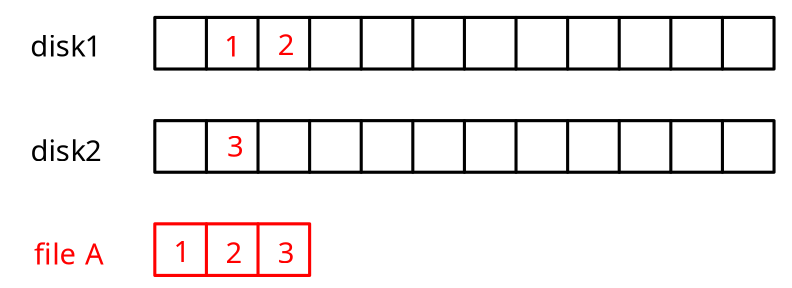
\includegraphics[scale=0.3]{img/RAID0.png}
    \end{figure}
    \paragraph{Caratteristiche} Analizziamo le caratteristiche di questa gestione:
    \begin{enumerate}
        \item Aumento della banda.
        \item Nessuna garanzia sull'affidabilità, anzi la peggioro, dato che il fault di un disco comprometterebbe tutto data la distribuzione dei file data dallo striping.
    \end{enumerate}
    \vspace*{10px}
    \item \textbf{RAID 1}: Si utilizza il \textbf{mirroring} \textbf{senza} alcun tipo di \textbf{correzione}:
    \begin{figure}[htbp]
        \center
        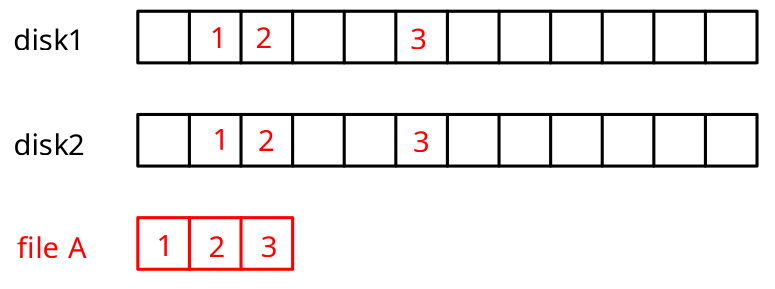
\includegraphics[scale=0.3]{img/RAID1.png}
    \end{figure}

\newpage

    \paragraph{Caratteristiche} Analizziamo le caratteristiche di questa gestione:
    \begin{enumerate}
        \item Posso risolvere un fault di disco "facilmente", ipotizziamo ad esempio il fault di $disk1$, potrei sostituire quest'ultimo con un $disk1'$ e
        riportare tutto in mirroring.
        \item Diminuzione della banda, questo varia in base al tipo di gestione di RAID 1:
        \begin{enumerate}
            \item \textbf{Soluzione Hardware + Software}: L'operazione costerebbe i tempi di $2$ init ed $1$ exec.
            \item \textbf{Soluzione solo Hardware}: Un componente specifico RAID si occuperebbe della gestione delle operazioni, di conseguenza
            il costo corrisponderebbe ad i tempi di $1$ init, $2$ init HW ed $1$ exec.
            \item \textbf{Soluzione solo Software}: Un operazione corrisponderebbe a due operazioni su due File System diversi.
        \end{enumerate}
        \item Un fault verrebbe dunque così gestito:
        \begin{enumerate}
            \item \textbf{Soluzione solo Hardware}: Tutte le locazioni contrassegnate come "BAD" in un disco vengono specchiate anche sugli altri.
            \begin{figure}[htbp]
                \center
                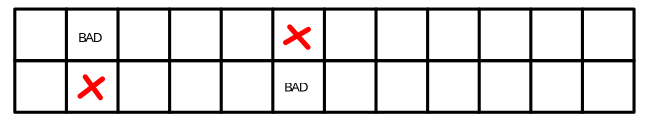
\includegraphics[scale=0.35]{img/fault_RAID1.png}
            \end{figure}
            \item \textbf{Soluzione solo Software}: Il problema del mirroring delle locazioni contrassegnate come "BAD" non occorre, dato che tutto viene gestito da specifico FS.
        \end{enumerate}
    \end{enumerate}
    \item \textbf{RAID 2/3}: Si basano sull'utilizzo dello \textbf{striping} a livello di \textbf{bit} e \textbf{byte}, seguono uno schema di \textbf{scrittura circolare} (utilizzo del modulo) su disco e usano codici di correzione di errori con \textbf{Hamming}. 
    \item \textbf{RAID 4}: Si basa sull'utilizzo di \textbf{block striping} e \textbf{dedicated parity}.
    \item \textbf{RAID 5}: Si basa sull'utilizzo di striping di blocco e codici d'errore:
    
    \begin{figure}[htbp]
        \center
        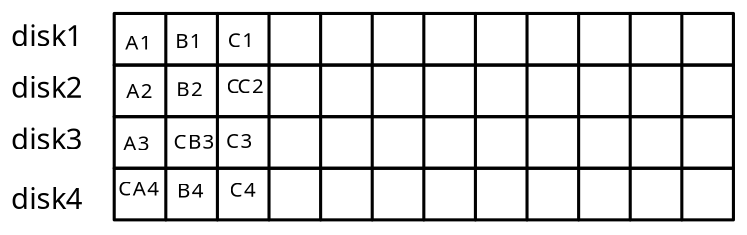
\includegraphics[scale=0.3]{img/RAID5.png}
    \end{figure}

    Questi codici di \textbf{correzione} si basano sull'utilizzo dello $xor$, se l'ipotesi della distribuzione omogenea è mantenuta allora nel caso in cui occorresse il fault di un disco saremmo in grado di \textbf{riottenere facilmente le informazioni perse}. Ad esempio, assumendo che nel $disk3$ avvenga un fault:
    \[ A_{1} \: xor \: A_{2} \: xor \: A_{3} = CA_{123} \Leftrightarrow A_{3} = A_{1} \: xor \: A_{2} \: xor \: CA_{123} \]

\newpage

    \paragraph{Caratteristiche} Analizziamo le caratteristiche di questa gestione:
    \begin{enumerate}
        \item \textbf{Performance}: Peggiora la banda $\approx 33\%$ dato che le info sono tutte in $xor$.
        \item \textbf{Affidabilità}: Ho un buon livello di affidabilità garantita.
    \end{enumerate}

    \item \textbf{RAID 6}: Come nello schema precedente vengono utilizzati codici di controllo in $xor$, che però in questo caso vengono duplicati e collocati
    su dischi diversi. Di conseguenza si otterrà un ulteriore perdita di banda ma ottime garanzie sull'affidabilità.

    \item \textbf{RAID 1-0}: Schema basato su un RAID0 di blocchi in RAID1. Questa combinazione ci permette di garantire una buona capacità grazie al RAID 0 ed una buona affidabilità grazie al RAID 0.
    Un esempio potrebbe essere:
    
    \begin{enumerate}
        \item \textbf{Blocco 1}: $disk1$ e $disk2$ tra loro in RAID1, dunque gestiti tra loro in mirroring.
        \item \textbf{Blocco 2}: $disk3$ e $disk4$ tra loro in RAID1, dunque gestiti tra loro in mirroring. 
    \end{enumerate}
    
    Questi due blocchi $Blocco1$ e $Blocco2$ sono tra loro in RAID0, dunque in gestiti tra loro in striping.

\end{enumerate}

\newpage

\end{document}